% Options for packages loaded elsewhere
\PassOptionsToPackage{unicode}{hyperref}
\PassOptionsToPackage{hyphens}{url}
\PassOptionsToPackage{dvipsnames,svgnames*,x11names*}{xcolor}
%
\documentclass[
]{article}
\usepackage{amsmath,amssymb}
\usepackage{lmodern}
\usepackage{ifxetex,ifluatex}
\ifnum 0\ifxetex 1\fi\ifluatex 1\fi=0 % if pdftex
  \usepackage[T1]{fontenc}
  \usepackage[utf8]{inputenc}
  \usepackage{textcomp} % provide euro and other symbols
\else % if luatex or xetex
  \usepackage{unicode-math}
  \defaultfontfeatures{Scale=MatchLowercase}
  \defaultfontfeatures[\rmfamily]{Ligatures=TeX,Scale=1}
\fi
% Use upquote if available, for straight quotes in verbatim environments
\IfFileExists{upquote.sty}{\usepackage{upquote}}{}
\IfFileExists{microtype.sty}{% use microtype if available
  \usepackage[]{microtype}
  \UseMicrotypeSet[protrusion]{basicmath} % disable protrusion for tt fonts
}{}
\makeatletter
\@ifundefined{KOMAClassName}{% if non-KOMA class
  \IfFileExists{parskip.sty}{%
    \usepackage{parskip}
  }{% else
    \setlength{\parindent}{0pt}
    \setlength{\parskip}{6pt plus 2pt minus 1pt}}
}{% if KOMA class
  \KOMAoptions{parskip=half}}
\makeatother
\usepackage{xcolor}
\IfFileExists{xurl.sty}{\usepackage{xurl}}{} % add URL line breaks if available
\IfFileExists{bookmark.sty}{\usepackage{bookmark}}{\usepackage{hyperref}}
\hypersetup{
  pdftitle={ggstatsplot: ggplot2 Based Plots with Statistical Details},
  pdfauthor={Indrajeet Patil},
  colorlinks=true,
  linkcolor=blue,
  filecolor=Maroon,
  citecolor=Blue,
  urlcolor=Blue,
  pdfcreator={LaTeX via pandoc}}
\urlstyle{same} % disable monospaced font for URLs
\usepackage[margin=1in]{geometry}
\usepackage{color}
\usepackage{fancyvrb}
\newcommand{\VerbBar}{|}
\newcommand{\VERB}{\Verb[commandchars=\\\{\}]}
\DefineVerbatimEnvironment{Highlighting}{Verbatim}{commandchars=\\\{\}}
% Add ',fontsize=\small' for more characters per line
\usepackage{framed}
\definecolor{shadecolor}{RGB}{248,248,248}
\newenvironment{Shaded}{\begin{snugshade}}{\end{snugshade}}
\newcommand{\AlertTok}[1]{\textcolor[rgb]{0.94,0.16,0.16}{#1}}
\newcommand{\AnnotationTok}[1]{\textcolor[rgb]{0.56,0.35,0.01}{\textbf{\textit{#1}}}}
\newcommand{\AttributeTok}[1]{\textcolor[rgb]{0.77,0.63,0.00}{#1}}
\newcommand{\BaseNTok}[1]{\textcolor[rgb]{0.00,0.00,0.81}{#1}}
\newcommand{\BuiltInTok}[1]{#1}
\newcommand{\CharTok}[1]{\textcolor[rgb]{0.31,0.60,0.02}{#1}}
\newcommand{\CommentTok}[1]{\textcolor[rgb]{0.56,0.35,0.01}{\textit{#1}}}
\newcommand{\CommentVarTok}[1]{\textcolor[rgb]{0.56,0.35,0.01}{\textbf{\textit{#1}}}}
\newcommand{\ConstantTok}[1]{\textcolor[rgb]{0.00,0.00,0.00}{#1}}
\newcommand{\ControlFlowTok}[1]{\textcolor[rgb]{0.13,0.29,0.53}{\textbf{#1}}}
\newcommand{\DataTypeTok}[1]{\textcolor[rgb]{0.13,0.29,0.53}{#1}}
\newcommand{\DecValTok}[1]{\textcolor[rgb]{0.00,0.00,0.81}{#1}}
\newcommand{\DocumentationTok}[1]{\textcolor[rgb]{0.56,0.35,0.01}{\textbf{\textit{#1}}}}
\newcommand{\ErrorTok}[1]{\textcolor[rgb]{0.64,0.00,0.00}{\textbf{#1}}}
\newcommand{\ExtensionTok}[1]{#1}
\newcommand{\FloatTok}[1]{\textcolor[rgb]{0.00,0.00,0.81}{#1}}
\newcommand{\FunctionTok}[1]{\textcolor[rgb]{0.00,0.00,0.00}{#1}}
\newcommand{\ImportTok}[1]{#1}
\newcommand{\InformationTok}[1]{\textcolor[rgb]{0.56,0.35,0.01}{\textbf{\textit{#1}}}}
\newcommand{\KeywordTok}[1]{\textcolor[rgb]{0.13,0.29,0.53}{\textbf{#1}}}
\newcommand{\NormalTok}[1]{#1}
\newcommand{\OperatorTok}[1]{\textcolor[rgb]{0.81,0.36,0.00}{\textbf{#1}}}
\newcommand{\OtherTok}[1]{\textcolor[rgb]{0.56,0.35,0.01}{#1}}
\newcommand{\PreprocessorTok}[1]{\textcolor[rgb]{0.56,0.35,0.01}{\textit{#1}}}
\newcommand{\RegionMarkerTok}[1]{#1}
\newcommand{\SpecialCharTok}[1]{\textcolor[rgb]{0.00,0.00,0.00}{#1}}
\newcommand{\SpecialStringTok}[1]{\textcolor[rgb]{0.31,0.60,0.02}{#1}}
\newcommand{\StringTok}[1]{\textcolor[rgb]{0.31,0.60,0.02}{#1}}
\newcommand{\VariableTok}[1]{\textcolor[rgb]{0.00,0.00,0.00}{#1}}
\newcommand{\VerbatimStringTok}[1]{\textcolor[rgb]{0.31,0.60,0.02}{#1}}
\newcommand{\WarningTok}[1]{\textcolor[rgb]{0.56,0.35,0.01}{\textbf{\textit{#1}}}}
\usepackage{longtable,booktabs,array}
\usepackage{calc} % for calculating minipage widths
% Correct order of tables after \paragraph or \subparagraph
\usepackage{etoolbox}
\makeatletter
\patchcmd\longtable{\par}{\if@noskipsec\mbox{}\fi\par}{}{}
\makeatother
% Allow footnotes in longtable head/foot
\IfFileExists{footnotehyper.sty}{\usepackage{footnotehyper}}{\usepackage{footnote}}
\makesavenoteenv{longtable}
\usepackage{graphicx}
\makeatletter
\def\maxwidth{\ifdim\Gin@nat@width>\linewidth\linewidth\else\Gin@nat@width\fi}
\def\maxheight{\ifdim\Gin@nat@height>\textheight\textheight\else\Gin@nat@height\fi}
\makeatother
% Scale images if necessary, so that they will not overflow the page
% margins by default, and it is still possible to overwrite the defaults
% using explicit options in \includegraphics[width, height, ...]{}
\setkeys{Gin}{width=\maxwidth,height=\maxheight,keepaspectratio}
% Set default figure placement to htbp
\makeatletter
\def\fps@figure{htbp}
\makeatother
\setlength{\emergencystretch}{3em} % prevent overfull lines
\providecommand{\tightlist}{%
  \setlength{\itemsep}{0pt}\setlength{\parskip}{0pt}}
\setcounter{secnumdepth}{5}
\usepackage{amsmath}
\usepackage{amssymb}
\usepackage{longtable}
\usepackage{booktabs}
\usepackage{amsfonts}
\usepackage{hyperref}
\usepackage{booktabs}
\usepackage{float}
\usepackage[dvipsnames]{xcolor}
\usepackage{fontawesome}
\ifluatex
  \usepackage{selnolig}  % disable illegal ligatures
\fi
\newlength{\cslhangindent}
\setlength{\cslhangindent}{1.5em}
\newlength{\csllabelwidth}
\setlength{\csllabelwidth}{3em}
\newenvironment{CSLReferences}[2] % #1 hanging-ident, #2 entry spacing
 {% don't indent paragraphs
  \setlength{\parindent}{0pt}
  % turn on hanging indent if param 1 is 1
  \ifodd #1 \everypar{\setlength{\hangindent}{\cslhangindent}}\ignorespaces\fi
  % set entry spacing
  \ifnum #2 > 0
  \setlength{\parskip}{#2\baselineskip}
  \fi
 }%
 {}
\usepackage{calc}
\newcommand{\CSLBlock}[1]{#1\hfill\break}
\newcommand{\CSLLeftMargin}[1]{\parbox[t]{\csllabelwidth}{#1}}
\newcommand{\CSLRightInline}[1]{\parbox[t]{\linewidth - \csllabelwidth}{#1}\break}
\newcommand{\CSLIndent}[1]{\hspace{\cslhangindent}#1}

\title{ggstatsplot: ggplot2 Based Plots with Statistical Details}
\author{Indrajeet Patil\footnote{Max Planck Institute for Human Development, \href{mailto:patilindrajeet.science@gmail.com}{\nolinkurl{patilindrajeet.science@gmail.com}}}}
\date{2021-01-17}

\begin{document}
\maketitle

{
\hypersetup{linkcolor=}
\setcounter{tocdepth}{2}
\tableofcontents
}
\begin{quote}
``What is to be sought in designs for the display of information is the clear
portrayal of complexity. Not the complication of the simple; rather \ldots{} the
revelation of the complex.''\\
- Edward R. Tufte
\end{quote}

\hypertarget{introduction-raison-duxeatre}{%
\section{Introduction: Raison d'être}\label{introduction-raison-duxeatre}}

\href{https://indrajeetpatil.github.io/ggstatsplot/}{\texttt{ggstatsplot}} is an extension
of \href{https://github.com/tidyverse/ggplot2}{\texttt{ggplot2}} package for creating
graphics with details from statistical tests included in the plots themselves
and targeted primarily at behavioral sciences community to provide a one-line
code to produce information-rich plots. In a typical exploratory data analysis
workflow, data visualization and statistical modeling are two different phases:
visualization informs modeling, and modeling in its turn can suggest a
different visualization method, and so on and so forth. The central idea of
\texttt{ggstatsplot} is simple: combine these two phases into one in the form of
graphics with statistical details, which makes data exploration simpler and
faster.

\hypertarget{need-for-informative-visualizations}{%
\subsection{Need for informative visualizations}\label{need-for-informative-visualizations}}

\hypertarget{need-for-better-statistical-reporting}{%
\subsection{Need for better statistical reporting}\label{need-for-better-statistical-reporting}}

But why would combining statistical analysis with data visualization be helpful?
We list few reasons below-

\begin{itemize}
\tightlist
\item
  A recent survey (\protect\hyperlink{ref-nuijtenPrevalenceStatisticalReporting2016}{Nuijten, Hartgerink, van Assen, Epskamp, \& Wicherts, 2016}) revealed that
  one in eight papers in major psychology journals contained a grossly
  inconsistent \emph{p}-value that may have affected the statistical conclusion.
  \texttt{ggstatsplot} helps avoid such reporting errors: Since the plot and the
  statistical analysis are yoked together, the chances of making an error in
  reporting the results are minimized. One need not write the results manually
  or copy-paste them from a different statistics software program (like SPSS,
  SAS, and so on).
\end{itemize}

\hypertarget{ggstatsplot-at-a-glance}{%
\section{\texorpdfstring{\texttt{ggstatsplot} at a glance}{ggstatsplot at a glance}}\label{ggstatsplot-at-a-glance}}

\hypertarget{summary-of-types-of-plots-included}{%
\subsection{Summary of types of plots included}\label{summary-of-types-of-plots-included}}

It produces a limited kinds of ready-made plots for the supported analyses:

\begin{longtable}[]{@{}
  >{\raggedright\arraybackslash}p{(\columnwidth - 4\tabcolsep) * \real{0.21}}
  >{\raggedright\arraybackslash}p{(\columnwidth - 4\tabcolsep) * \real{0.29}}
  >{\raggedright\arraybackslash}p{(\columnwidth - 4\tabcolsep) * \real{0.50}}@{}}
\toprule
Function & Plot & Description \\ \addlinespace
\midrule
\endhead
\texttt{ggbetweenstats} & \textbf{violin plots} & for comparisons \emph{between} groups/conditions \\ \addlinespace
\texttt{ggwithinstats} & \textbf{violin plots} & for comparisons \emph{within} groups/conditions \\ \addlinespace
\texttt{gghistostats} & \textbf{histograms} & for distribution about numeric variable \\ \addlinespace
\texttt{ggdotplotstats} & \textbf{dot plots/charts} & for distribution about labeled numeric variable \\ \addlinespace
\texttt{ggscatterstats} & \textbf{scatterplots} & for correlation between two variables \\ \addlinespace
\texttt{ggcorrmat} & \textbf{correlation matrices} & for correlations between multiple variables \\ \addlinespace
\texttt{ggpiestats} & \textbf{pie charts} & for categorical data \\ \addlinespace
\texttt{ggbarstats} & \textbf{bar charts} & for categorical data \\ \addlinespace
\texttt{ggcoefstats} & \textbf{dot-and-whisker plots} & for regression models and meta-analysis \\ \addlinespace
\bottomrule
\end{longtable}

In addition to these basic plots, \texttt{ggstatsplot} also provides \textbf{\texttt{grouped\_}}
versions (see below) that makes it easy to repeat the same analysis for
any grouping variable.

\hypertarget{summary-of-types-of-statistical-analyses}{%
\subsection{Summary of types of statistical analyses}\label{summary-of-types-of-statistical-analyses}}

Most functions share a \texttt{type} (of test) argument that is helpful to specify the
type of statistical analysis:

\begin{itemize}
\tightlist
\item
  \texttt{"parametric"} (for \textbf{parametric} tests)
\item
  \texttt{"nonparametric"} (for \textbf{non-parametric} tests)
\item
  \texttt{"robust"} (for \textbf{robust} tests)
\item
  \texttt{"bayes"} (for \textbf{Bayes Factor} tests)
\end{itemize}

The table below summarizes all the different types of analyses
currently supported in this package-

\begin{longtable}[]{@{}
  >{\raggedright\arraybackslash}p{(\columnwidth - 10\tabcolsep) * \real{0.16}}
  >{\raggedright\arraybackslash}p{(\columnwidth - 10\tabcolsep) * \real{0.42}}
  >{\raggedright\arraybackslash}p{(\columnwidth - 10\tabcolsep) * \real{0.09}}
  >{\raggedright\arraybackslash}p{(\columnwidth - 10\tabcolsep) * \real{0.12}}
  >{\raggedright\arraybackslash}p{(\columnwidth - 10\tabcolsep) * \real{0.09}}
  >{\raggedright\arraybackslash}p{(\columnwidth - 10\tabcolsep) * \real{0.12}}@{}}
\toprule
Functions & Description & Parametric & Non-parametric & Robust & Bayesian \\ \addlinespace
\midrule
\endhead
\texttt{ggbetweenstats} & Between group/condition comparisons & \textcolor{ForestGreen}{Yes} & \textcolor{ForestGreen}{Yes} & \textcolor{ForestGreen}{Yes} & \textcolor{ForestGreen}{Yes} \\ \addlinespace
\texttt{ggwithinstats} & Within group/condition comparisons & \textcolor{ForestGreen}{Yes} & \textcolor{ForestGreen}{Yes} & \textcolor{ForestGreen}{Yes} & \textcolor{ForestGreen}{Yes} \\ \addlinespace
\texttt{gghistostats}, \texttt{ggdotplotstats} & Distribution of a numeric variable & \textcolor{ForestGreen}{Yes} & \textcolor{ForestGreen}{Yes} & \textcolor{ForestGreen}{Yes} & \textcolor{ForestGreen}{Yes} \\ \addlinespace
\texttt{ggcorrmat} & Correlation matrix & \textcolor{ForestGreen}{Yes} & \textcolor{ForestGreen}{Yes} & \textcolor{ForestGreen}{Yes} & \textcolor{ForestGreen}{Yes} \\ \addlinespace
\texttt{ggscatterstats} & Correlation between two variables & \textcolor{ForestGreen}{Yes} & \textcolor{ForestGreen}{Yes} & \textcolor{ForestGreen}{Yes} & \textcolor{ForestGreen}{Yes} \\ \addlinespace
\texttt{ggpiestats}, \texttt{ggbarstats} & Association between categorical variables & \textcolor{ForestGreen}{Yes} & \texttt{NA} & \texttt{NA} & \textcolor{ForestGreen}{Yes} \\ \addlinespace
\texttt{ggpiestats}, \texttt{ggbarstats} & Equal proportions for categorical variable levels & \textcolor{ForestGreen}{Yes} & \texttt{NA} & \texttt{NA} & \textcolor{ForestGreen}{Yes} \\ \addlinespace
\texttt{ggcoefstats} & Regression model coefficients & \textcolor{ForestGreen}{Yes} & \textcolor{ForestGreen}{Yes} & \textcolor{ForestGreen}{Yes} & \textcolor{ForestGreen}{Yes} \\ \addlinespace
\texttt{ggcoefstats} & Random-effects meta-analysis & \textcolor{ForestGreen}{Yes} & \texttt{NA} & \textcolor{ForestGreen}{Yes} & \textcolor{ForestGreen}{Yes} \\ \addlinespace
\bottomrule
\end{longtable}

In the following sections, we will discuss at depth justification for why the
plots have been designed in certain ways and what principles were followed to
report statistical details on the plots.

\hypertarget{graphic-design-principles}{%
\section{Graphic design principles}\label{graphic-design-principles}}

\hypertarget{graphical-perception}{%
\subsection{Graphical perception}\label{graphical-perception}}

Graphical perception involves visual decoding of the encoded information in
graphs. \texttt{ggstatsplot} incorporates the paradigm proposed in
((\protect\hyperlink{ref-clevelandElementsGraphingData1985}{Cleveland, 1985}), Chapter 4) to facilitate making visual
judgments about quantitative information effortless and almost instantaneous.
Based on experiments, Cleveland proposes that there are ten elementary
graphical-perception tasks that we perform to visually decode quantitative
information in graphs (organized from most to least accurate;
(\protect\hyperlink{ref-clevelandElementsGraphingData1985}{Cleveland, 1985}), p.254)-

\begin{itemize}
\tightlist
\item
  Position along a common scale
\item
  Position along identical, non-aligned scales
\item
  Length
\item
  Angle (Slope)
\item
  Area
\item
  Volume
\item
  Color hue
\end{itemize}

So the key principle of Cleveland's paradigm for data display is-

\begin{quote}
``We should encode data on a graph so that the visual decoding involves
{[}graphical-perception{]} tasks as high in the ordering as possible.''
\end{quote}

For example, decoding the data point values in \texttt{ggbetweenstats} requires
position judgments along a common scale (Figure \ref{fig:fig1}):

\begin{Shaded}
\begin{Highlighting}[]
\CommentTok{\# for reproducibility}
\FunctionTok{set.seed}\NormalTok{(}\DecValTok{123}\NormalTok{)}

\CommentTok{\# plot}
\NormalTok{ggstatsplot}\SpecialCharTok{::}\FunctionTok{ggbetweenstats}\NormalTok{(}
  \AttributeTok{data =}\NormalTok{ dplyr}\SpecialCharTok{::}\FunctionTok{filter}\NormalTok{(}
    \AttributeTok{.data =}\NormalTok{ ggstatsplot}\SpecialCharTok{::}\NormalTok{movies\_long,}
\NormalTok{    genre }\SpecialCharTok{\%in\%} \FunctionTok{c}\NormalTok{(}\StringTok{"Action"}\NormalTok{, }\StringTok{"Action Comedy"}\NormalTok{, }\StringTok{"Action Drama"}\NormalTok{, }\StringTok{"Comedy"}\NormalTok{)}
\NormalTok{  ),}
  \AttributeTok{x =}\NormalTok{ genre,}
  \AttributeTok{y =}\NormalTok{ rating,}
  \AttributeTok{title =} \StringTok{"IMDB rating by film genre"}\NormalTok{,}
  \AttributeTok{xlab =} \StringTok{"Genre"}\NormalTok{,}
  \AttributeTok{ylab =} \StringTok{"IMDB rating (average)"}\NormalTok{,}
  \AttributeTok{ggtheme =}\NormalTok{ hrbrthemes}\SpecialCharTok{::}\FunctionTok{theme\_ipsum\_tw}\NormalTok{(),}
  \AttributeTok{ggstatsplot.layer =} \ConstantTok{FALSE}\NormalTok{,}
  \AttributeTok{outlier.tagging =} \ConstantTok{TRUE}\NormalTok{,}
  \AttributeTok{outlier.label =}\NormalTok{ title}
\NormalTok{)}
\end{Highlighting}
\end{Shaded}

\begin{figure}[H]
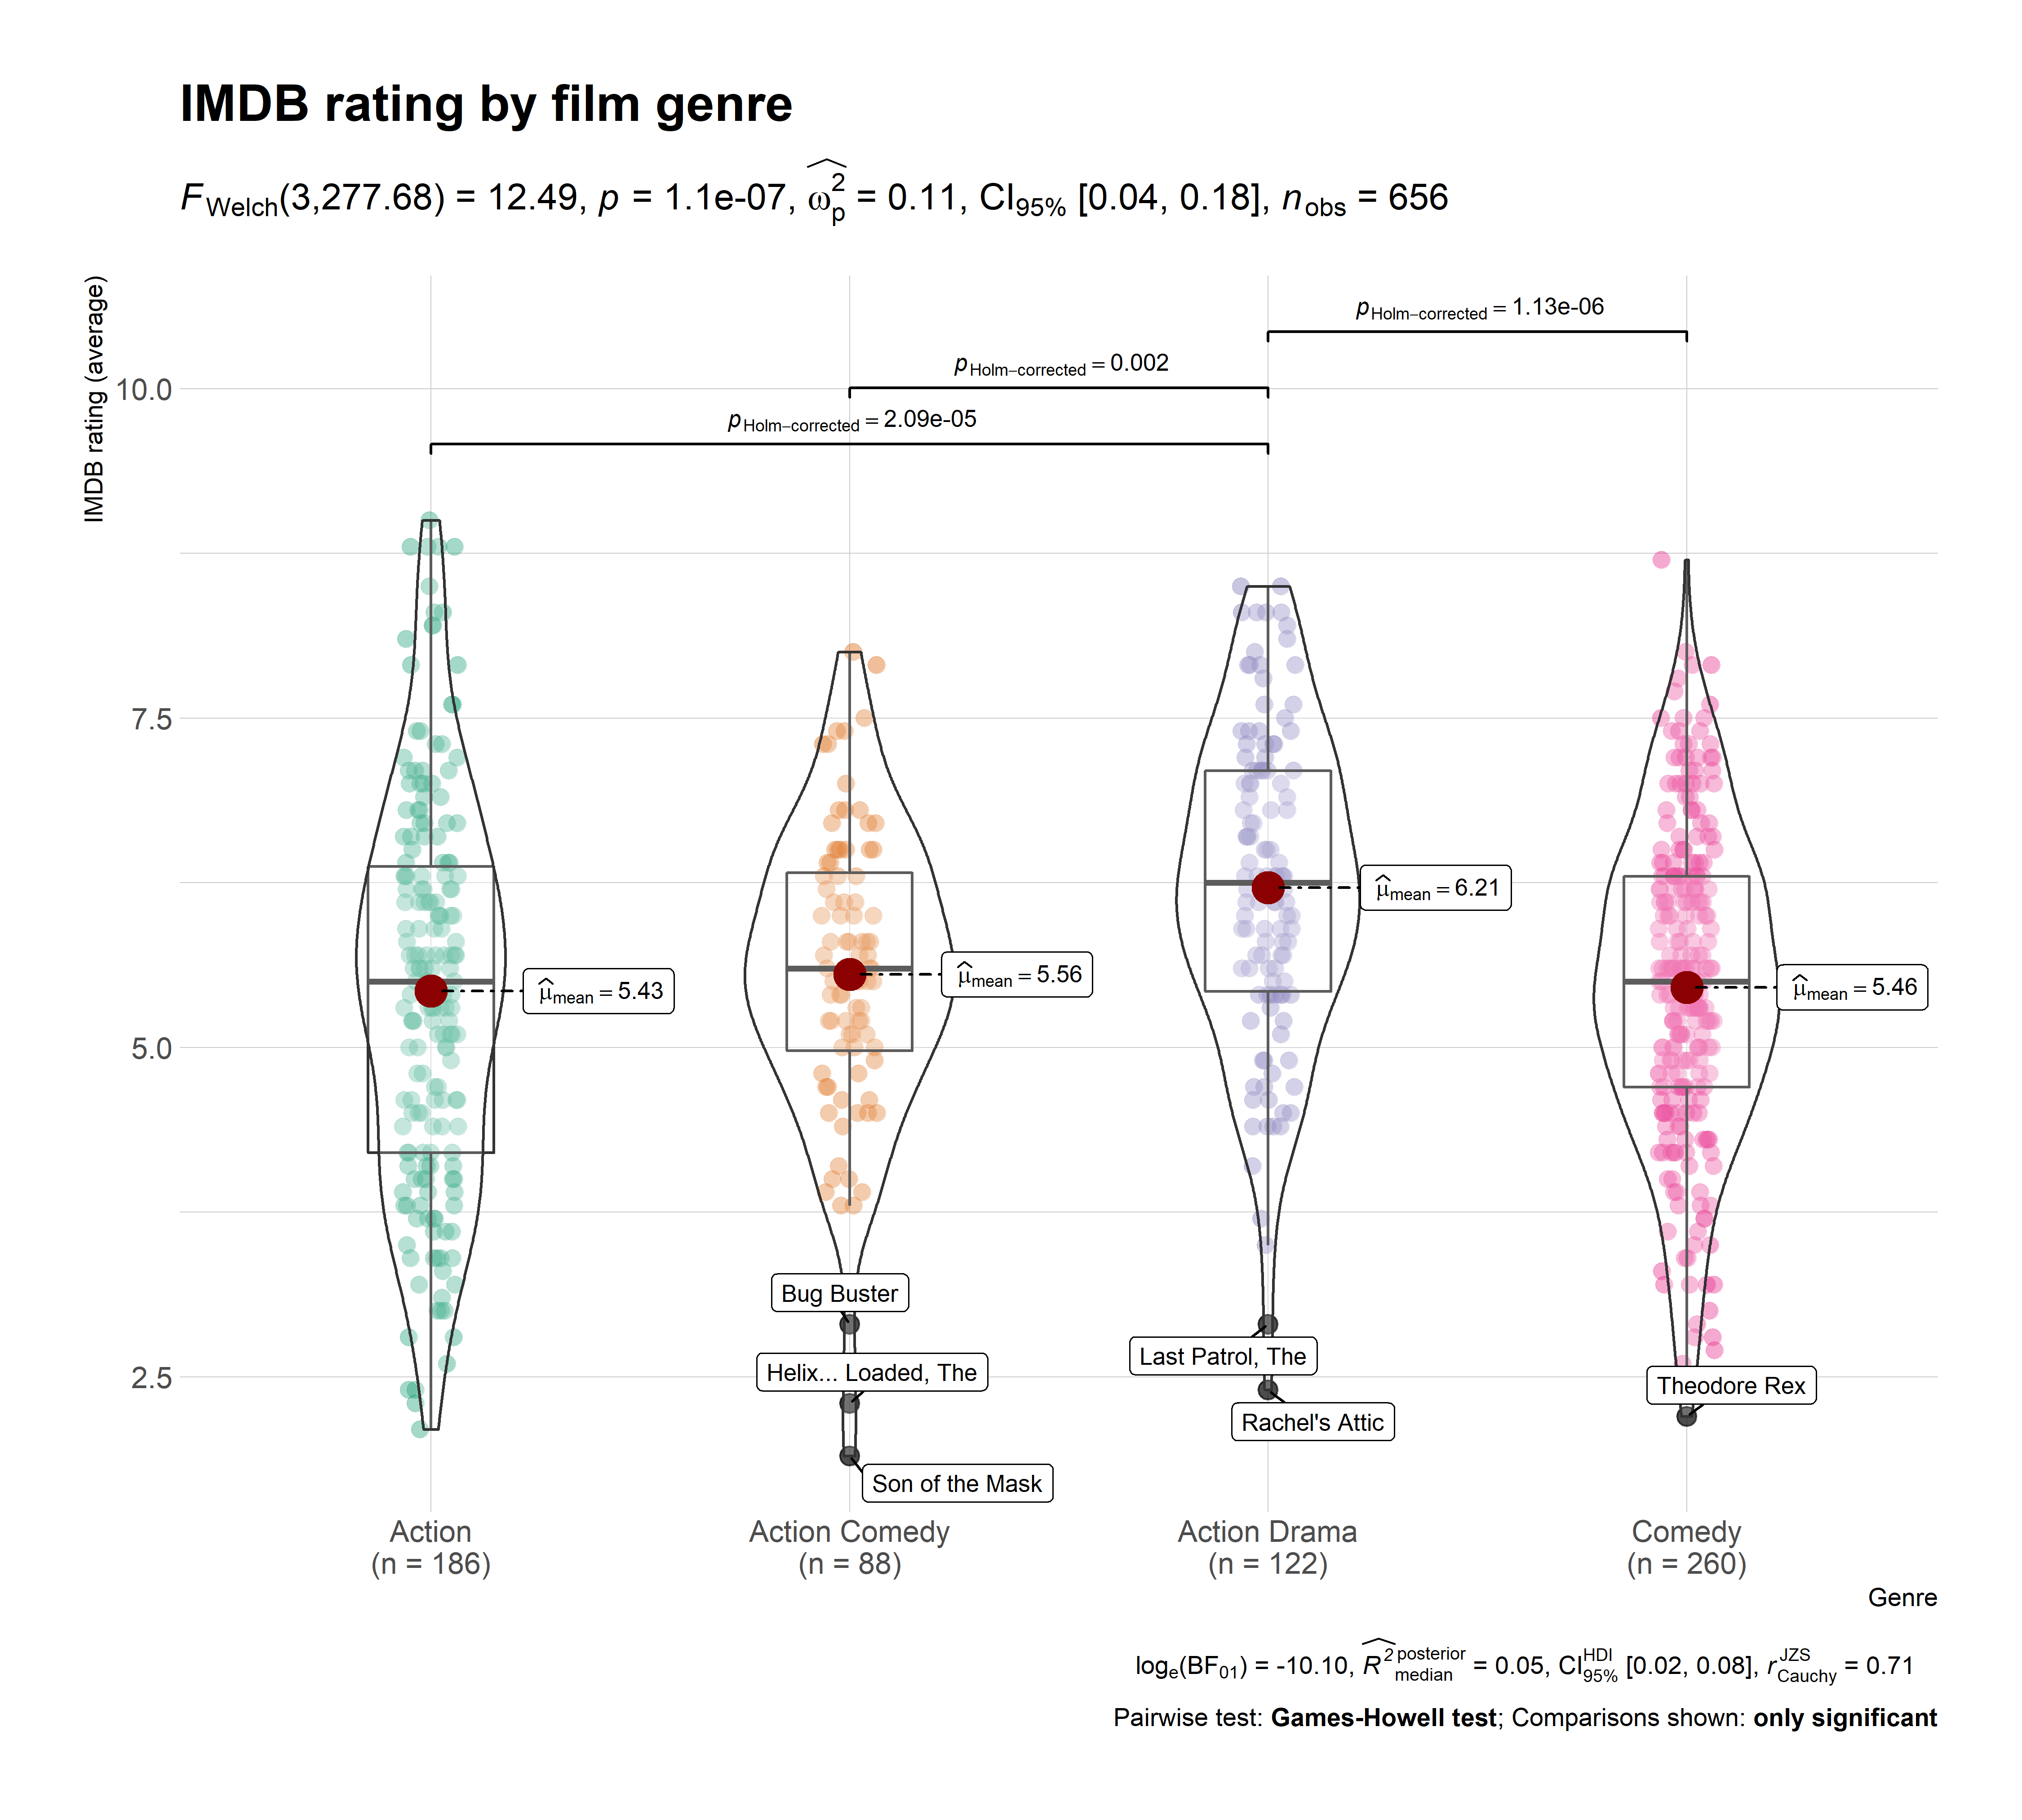
\includegraphics[width=1\linewidth]{./figures/paper-fig1-1} \caption{Note that assessing differences in mean values between groups has been made easier with the help of \textit{position} of data points along a common scale (the Y-axis) and labels.}\label{fig:fig1}
\end{figure}

There are few instances where \texttt{ggstatsplot} diverges from recommendations made
in Cleveland's paradigm:

\begin{itemize}
\tightlist
\item
  For the categorical/nominal data, \texttt{ggstatsplot} uses pie charts (see Figure
  \ref{fig:fig2}) which rely on \emph{angle} judgments, which are less accurate (as
  compared to bar graphs, e.g., which require \emph{position} judgments). This
  shortcoming is assuaged to some degree by using plenty of labels that
  describe percentages for all slices. This makes angle judgment unnecessary
  and pre-vacates any concerns about inaccurate judgments about percentages.
  Additionally, it also provides alternative function to \texttt{ggpiestats} for
  working with categorical variables: \texttt{ggbarstats}.
\end{itemize}

\begin{Shaded}
\begin{Highlighting}[]
\CommentTok{\# for reproducibility}
\FunctionTok{set.seed}\NormalTok{(}\DecValTok{123}\NormalTok{)}

\CommentTok{\# plot}
\NormalTok{ggstatsplot}\SpecialCharTok{::}\FunctionTok{ggpiestats}\NormalTok{(}
  \AttributeTok{data =}\NormalTok{ ggstatsplot}\SpecialCharTok{::}\NormalTok{movies\_long,}
  \AttributeTok{x =}\NormalTok{ genre,}
  \AttributeTok{y =}\NormalTok{ mpaa,}
  \AttributeTok{title =} \StringTok{"Distribution of MPAA ratings by film genre"}\NormalTok{,}
  \AttributeTok{legend.title =} \StringTok{"layout"}\NormalTok{,}
  \AttributeTok{caption =} \FunctionTok{substitute}\NormalTok{(}\FunctionTok{paste}\NormalTok{(}
    \FunctionTok{italic}\NormalTok{(}\StringTok{"MPAA"}\NormalTok{), }\StringTok{": Motion Picture Association of America"}
\NormalTok{  )),}
  \AttributeTok{palette =} \StringTok{"Paired"}
\NormalTok{)}
\end{Highlighting}
\end{Shaded}

\begin{figure}[H]
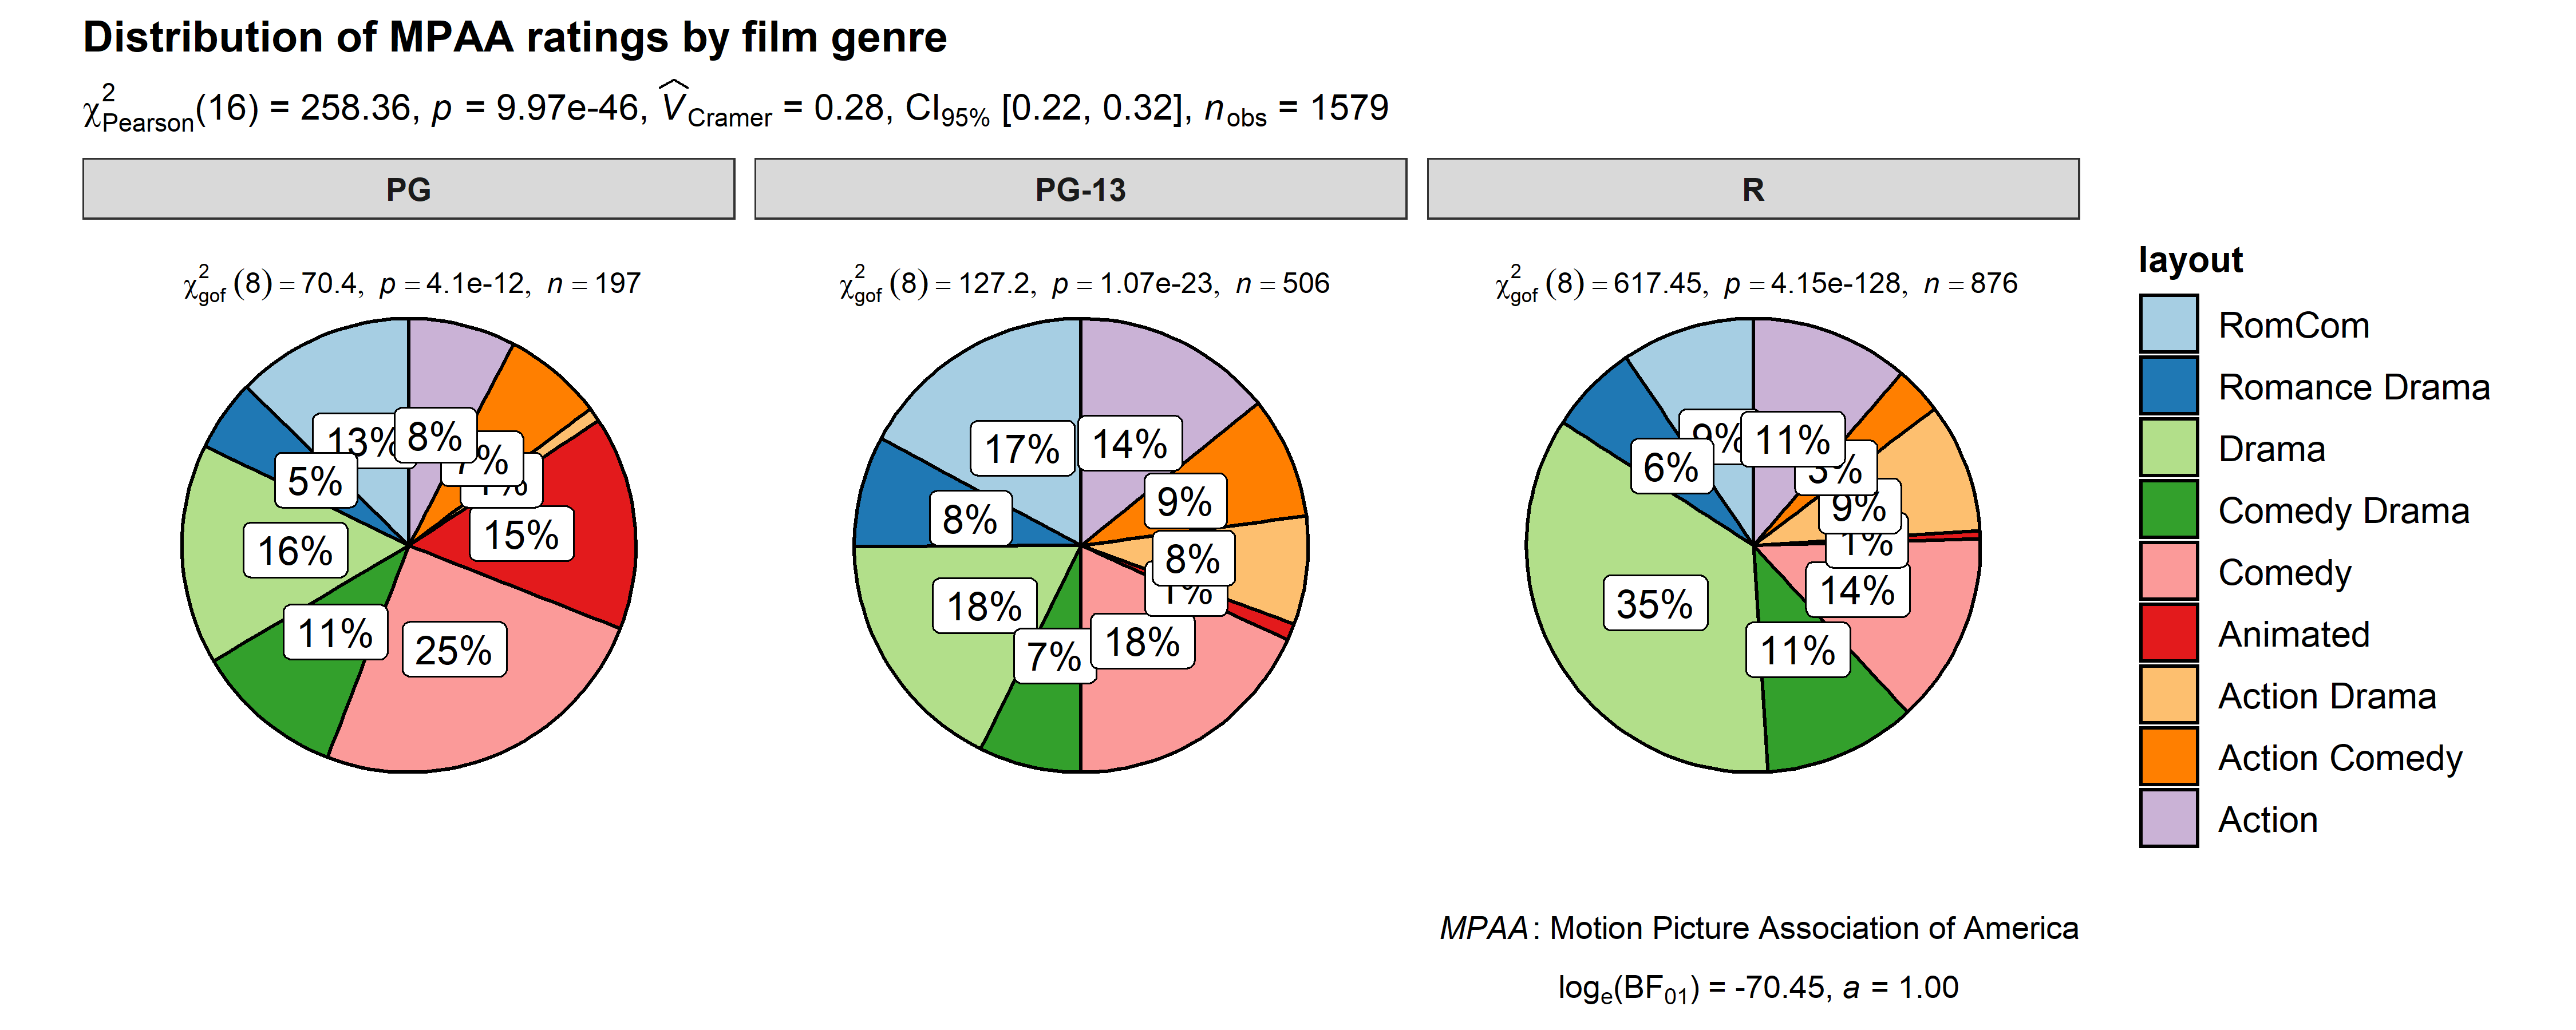
\includegraphics[width=1\linewidth]{./figures/paper-fig2-1} \caption{Pie charts don't follow Cleveland's paradigm to data display because they rely on less accurate angle judgments. `ggstatsplot` sidesteps this issue by always labelling percentages for pie slices, which makes angle judgments unnecessary.}\label{fig:fig2}
\end{figure}

\begin{itemize}
\tightlist
\item
  Cleveland's paradigm also emphasizes that \emph{superposition} of data is better
  than \emph{juxtaposition} ((\protect\hyperlink{ref-clevelandElementsGraphingData1985}{Cleveland, 1985}), p.201) because
  this allows for a more incisive comparison of the values from different
  parts of the dataset. This recommendation is violated in all \texttt{grouped\_}
  variants of the function (see Figure \ref{fig:fig3}). Note that the range
  for Y-axes are no longer the same across juxtaposed subplots and so visually
  comparing the data becomes difficult. On the other hand, in the superposed
  plot, all data have the same range and coloring different parts makes the
  visual discrimination of different components of the data, and their
  comparison, easier. But the goal of \texttt{grouped\_} variants of functions is to
  not only show different aspects of the data but also to run statistical
  tests and showing detailed results for all aspects of the data in a
  superposed plot is difficult. Therefore, this is a compromise \texttt{ggstatsplot}
  is comfortable with, at least to produce plots for quick exploration of
  different aspects of the data.
\end{itemize}

\begin{Shaded}
\begin{Highlighting}[]
\CommentTok{\# for reproducibility}
\FunctionTok{set.seed}\NormalTok{(}\DecValTok{123}\NormalTok{)}
\FunctionTok{library}\NormalTok{(ggplot2)}

\CommentTok{\# creating a smaller dataframe}
\NormalTok{df }\OtherTok{\textless{}{-}}\NormalTok{ dplyr}\SpecialCharTok{::}\FunctionTok{filter}\NormalTok{(ggstatsplot}\SpecialCharTok{::}\NormalTok{movies\_long, genre }\SpecialCharTok{\%in\%} \FunctionTok{c}\NormalTok{(}\StringTok{"Comedy"}\NormalTok{, }\StringTok{"Drama"}\NormalTok{))}

\CommentTok{\# plot}
\NormalTok{ggstatsplot}\SpecialCharTok{::}\FunctionTok{combine\_plots}\NormalTok{(}
  \CommentTok{\# plot 1: superposition}
  \FunctionTok{ggplot}\NormalTok{(}\AttributeTok{data =}\NormalTok{ df, }\AttributeTok{mapping =}\NormalTok{ ggplot2}\SpecialCharTok{::}\FunctionTok{aes}\NormalTok{(}\AttributeTok{x =}\NormalTok{ length, }\AttributeTok{y =}\NormalTok{ rating, }\AttributeTok{color =}\NormalTok{ genre)) }\SpecialCharTok{+}
    \FunctionTok{geom\_jitter}\NormalTok{(}\AttributeTok{size =} \DecValTok{3}\NormalTok{, }\AttributeTok{alpha =} \FloatTok{0.5}\NormalTok{) }\SpecialCharTok{+}
    \FunctionTok{geom\_smooth}\NormalTok{(}\AttributeTok{method =} \StringTok{"lm"}\NormalTok{) }\SpecialCharTok{+}
    \FunctionTok{labs}\NormalTok{(}\AttributeTok{title =} \StringTok{"superposition (recommended in Cleveland\textquotesingle{}s paradigm)"}\NormalTok{) }\SpecialCharTok{+}
\NormalTok{    ggstatsplot}\SpecialCharTok{::}\FunctionTok{theme\_ggstatsplot}\NormalTok{(),}
  \CommentTok{\# plot 2: juxtaposition}
\NormalTok{  ggstatsplot}\SpecialCharTok{::}\FunctionTok{grouped\_ggscatterstats}\NormalTok{(}
    \AttributeTok{data =}\NormalTok{ df,}
    \AttributeTok{x =}\NormalTok{ length,}
    \AttributeTok{y =}\NormalTok{ rating,}
    \AttributeTok{grouping.var =}\NormalTok{ genre,}
    \AttributeTok{marginal =} \ConstantTok{FALSE}\NormalTok{,}
    \AttributeTok{title.prefix =} \StringTok{"Genre"}\NormalTok{,}
    \AttributeTok{title.text =} \StringTok{"juxtaposition (\textasciigrave{}ggstatsplot\textasciigrave{} implementation in \textasciigrave{}grouped\_\textasciigrave{} functions)"}\NormalTok{,}
    \AttributeTok{title.size =} \DecValTok{12}
\NormalTok{  ),}
  \CommentTok{\# combine for comparison}
  \AttributeTok{title.text =} \StringTok{"Two ways to compare different aspects of data"}\NormalTok{,}
  \AttributeTok{nrow =} \DecValTok{2}\NormalTok{,}
  \AttributeTok{labels =} \FunctionTok{c}\NormalTok{(}\StringTok{"(a)"}\NormalTok{, }\StringTok{"(b)"}\NormalTok{)}
\NormalTok{)}
\end{Highlighting}
\end{Shaded}

\begin{figure}[H]
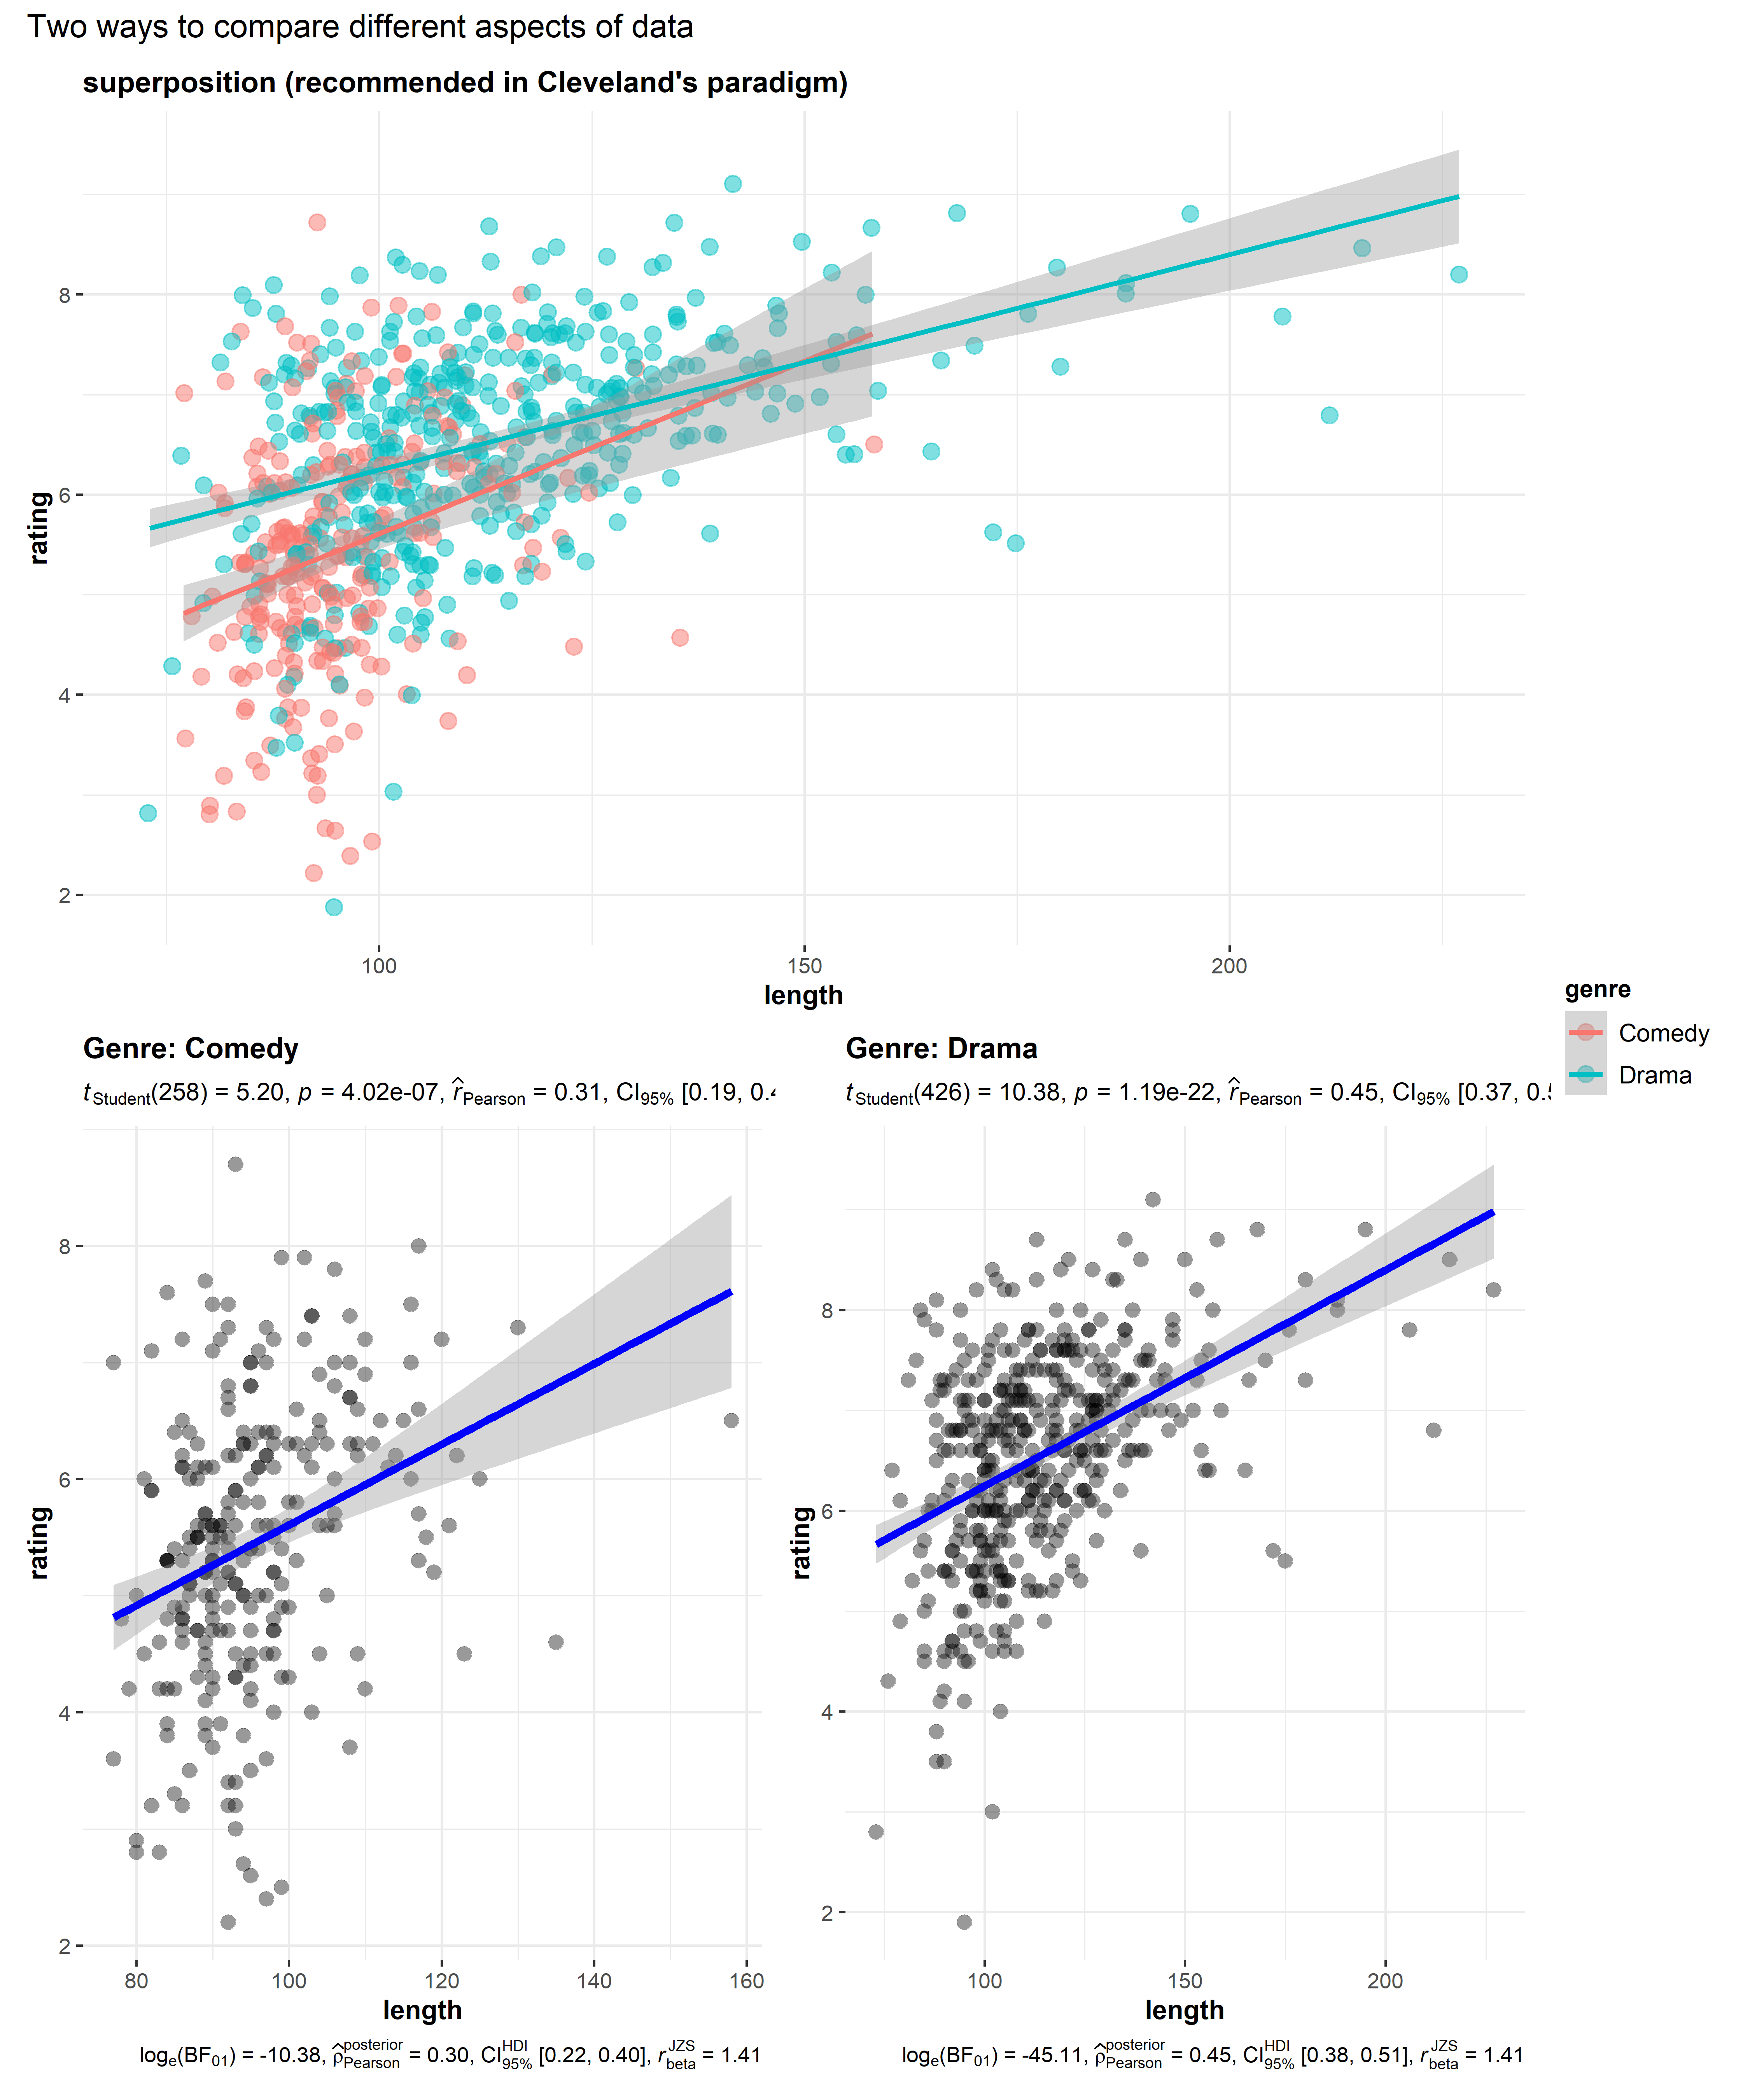
\includegraphics[width=1\linewidth]{./figures/paper-fig3-1} \caption{Comparing different aspects of data is much more accurate in (\textit{a}) a \textit{superposed} plot, which is recommended in Cleveland's paradigm, than in (\textit{b}) a \textit{juxtaposed} plot, which is how it is implemented in `ggstatsplot` package. This is because displaying detailed results from statistical tests would be difficult in a superposed plot.}\label{fig:fig3}
\end{figure}

The \texttt{grouped\_} plots follow the \emph{Shrink Principle}
((\protect\hyperlink{ref-tufteVisualDisplayQuantitative2001}{Tufte, 2001}), p.166-7) for high-information graphics,
which dictates that the data density and the size of the data matrix can be
maximized to exploit maximum resolution of the available data-display
technology. Given the large maximum resolution afforded by most computer
monitors today, saving \texttt{grouped\_} plots with appropriate resolution ensures no
loss in legibility with reduced graphics area.

\hypertarget{graphical-excellence}{%
\subsection{Graphical excellence}\label{graphical-excellence}}

Graphical excellence consists of communicating complex ideas with clarity and in
a way that the viewer understands the greatest number of ideas in a short amount
of time all the while not quoting the data out of context. The package follows
the principles for \emph{graphical integrity} (\protect\hyperlink{ref-tufteVisualDisplayQuantitative2001}{Tufte, 2001}):

\begin{itemize}
\item
  The physical representation of numbers is proportional to the numerical
  quantities they represent (e.g., Figure \ref{fig:fig1} and Figure
  \ref{fig:fig2} show how means (in \texttt{ggbetweenstats}) or percentages
  (\texttt{ggpiestats}) are proportional to the vertical distance or the area,
  respectively).
\item
  All important events in the data have clear, detailed, and thorough labeling
  (e.g., Figure \ref{fig:fig1} plot shows how \texttt{ggbetweenstats} labels means,
  sample size information, outliers, and pairwise comparisons; same can be
  appreciated for \texttt{ggpiestats} in Figure \ref{fig:fig2} and \texttt{gghistostats} in
  Figure \ref{fig:fig5}). Note that data labels in the data region are
  designed in a way that they don't interfere with our ability to assess the
  overall pattern of the data ((\protect\hyperlink{ref-clevelandElementsGraphingData1985}{Cleveland, 1985});
  p.44-45). This is achieved by using \texttt{ggrepel} package to place labels in a
  way that reduces their visual prominence.
\item
  None of the plots have \emph{design} variation (e.g., abrupt change in scales)
  over the surface of a same graphic because this can lead to a false
  impression about variation in \emph{data}.
\item
  The number of information-carrying dimensions never exceed the number of
  dimensions in the data (e.g., using area to show one-dimensional data).
\item
  All plots are designed to have no \textbf{chartjunk} (like moiré vibrations, fake
  perspective, dark grid lines, etc.)
  ((\protect\hyperlink{ref-tufteVisualDisplayQuantitative2001}{Tufte, 2001}), Chapter 5).
\end{itemize}

There are some instances where \texttt{ggstatsplot} graphs don't follow principles of
clean graphics, as formulated in the Tufte theory of data graphics
((\protect\hyperlink{ref-tufteVisualDisplayQuantitative2001}{Tufte, 2001}), Chapter 4). The theory has four key
principles:

\begin{enumerate}
\def\labelenumi{\arabic{enumi}.}
\tightlist
\item
  Above all else show the data.
\item
  Maximize the data-ink ratio.
\item
  Erase non-data-ink.
\item
  Erase redundant data-ink, within reason.
\end{enumerate}

In particular, default plots in \texttt{ggstatsplot} can sometimes violate one of the
principles from 2-4. According to these principles, every bit of ink should have
reason for its inclusion in the graphic and should convey some new information
to the viewer. If not, such ink should be removed. One instance of this is
bilateral symmetry of data measures. For example, in Figure \ref{fig:fig1}, we
can see that both the box and violin plots are mirrored, which consumes twice
the space in the graphic without adding any new information. But this redundancy
is tolerated for the sake of beauty that such symmetrical shapes can bring to
the graphic. Even Tufte admits that efficiency is but one consideration in the
design of statistical graphics ((\protect\hyperlink{ref-tufteVisualDisplayQuantitative2001}{Tufte, 2001}),
p.~137). Additionally, these principles were formulated in an era in which
computer graphics had yet to revolutionize the ease with which graphics could be
produced and thus some of the concerns about minimizing data-ink for easier
production of graphics are not as relevant as they were.

\hypertarget{statistical-variation}{%
\subsection{Statistical variation}\label{statistical-variation}}

One of the important functions of a plot is to show the variation in the data,
which comes in two forms:

\begin{itemize}
\tightlist
\item
  \textbf{Measurement noise}: In \texttt{ggstatsplot}, the actual variation in
  measurements is shown by plotting a combination of (jittered) raw data
  points with a boxplot laid on top (Figure \ref{fig:fig1}) or a histogram
  (Figure \ref{fig:fig5}). None of the plots, where empirical distribution of
  the data is concerned, show the sample standard deviation because they are
  poor at conveying information about limits of the sample and presence of
  outliers ((\protect\hyperlink{ref-clevelandElementsGraphingData1985}{Cleveland, 1985}), p.220).
\end{itemize}

\begin{Shaded}
\begin{Highlighting}[]
\CommentTok{\# for reproducibility}
\FunctionTok{set.seed}\NormalTok{(}\DecValTok{123}\NormalTok{)}

\CommentTok{\# plot}
\NormalTok{ggstatsplot}\SpecialCharTok{::}\FunctionTok{gghistostats}\NormalTok{(}
  \AttributeTok{data =}\NormalTok{ morley,}
  \AttributeTok{x =}\NormalTok{ Speed,}
  \AttributeTok{test.value =} \DecValTok{792}\NormalTok{,}
  \AttributeTok{xlab =} \StringTok{"Speed of light (km/sec, with 299000 subtracted)"}\NormalTok{,}
  \AttributeTok{title =} \StringTok{"Distribution of measured Speed of light"}\NormalTok{,}
  \AttributeTok{caption =} \StringTok{"Note: Data collected across 5 experiments (20 measurements each)"}
\NormalTok{)}
\end{Highlighting}
\end{Shaded}

\begin{figure}[H]
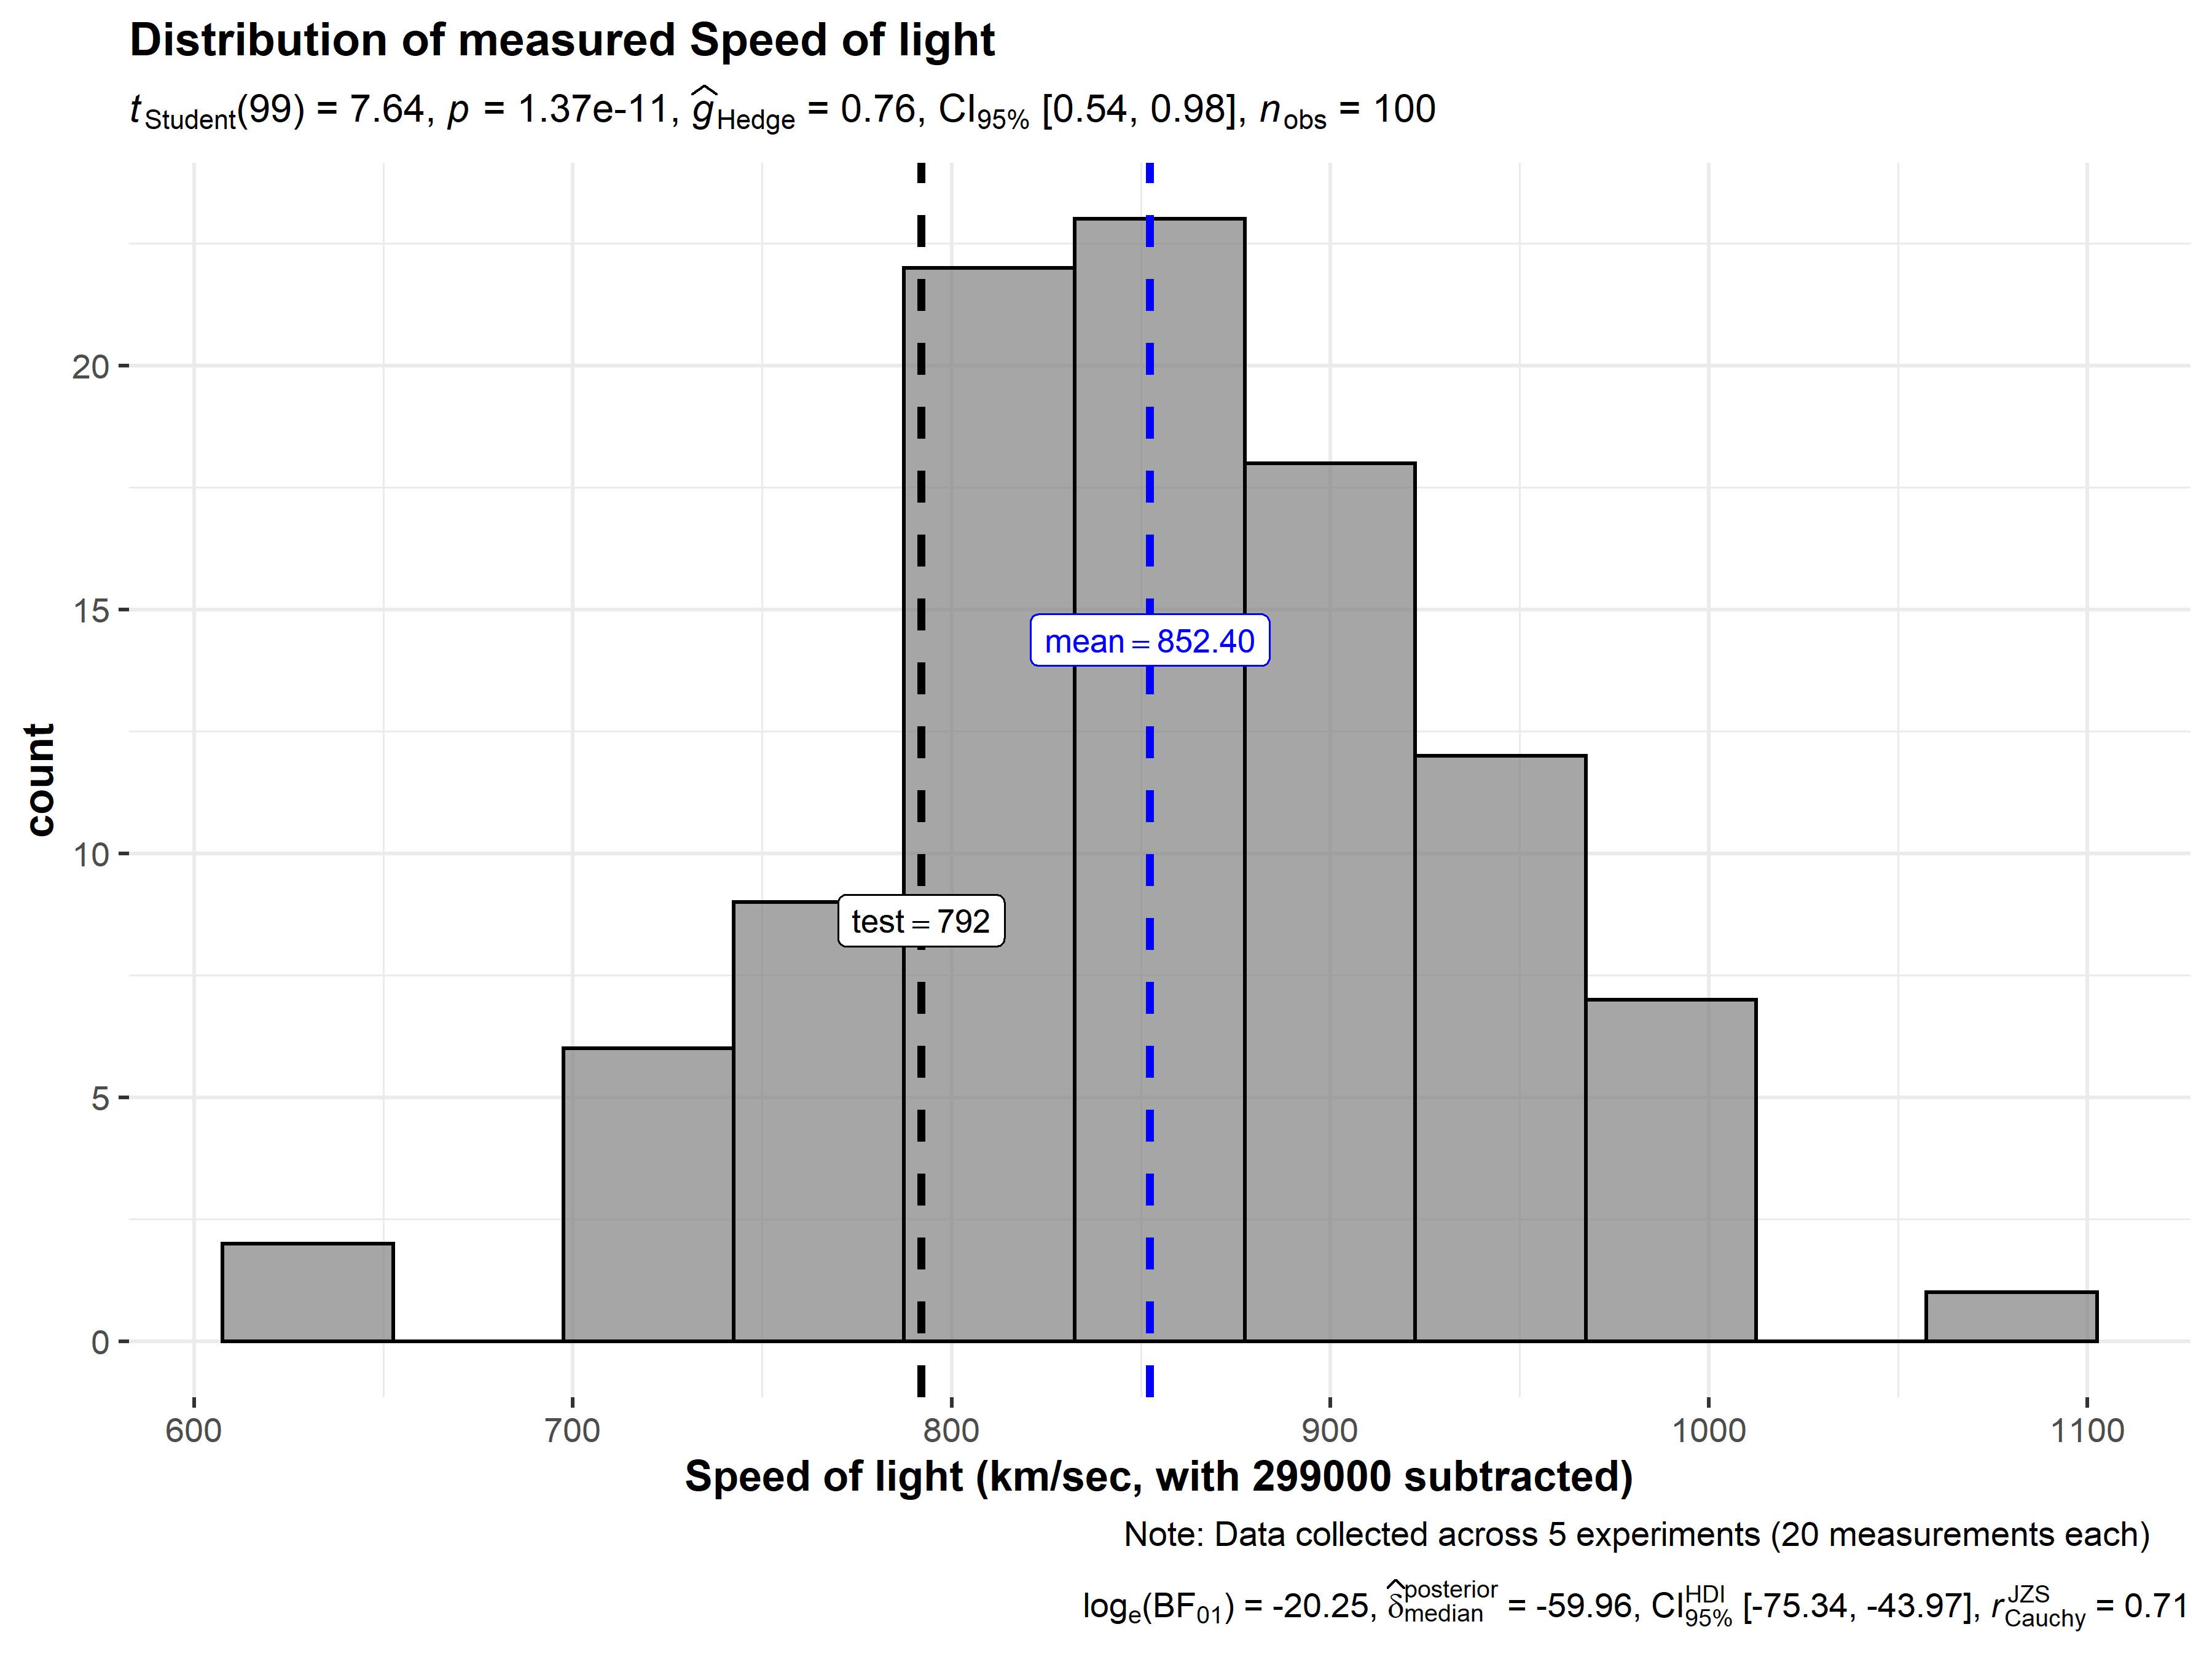
\includegraphics[width=1\linewidth]{./figures/paper-fig5-1} \caption{Distribution of a variable shown using `gghistostats`.}\label{fig:fig5}
\end{figure}

\begin{itemize}
\tightlist
\item
  \textbf{Sample-to-sample statistic variation}: Although, traditionally, this
  variation has been shown using the standard error of the mean (SEM) of the
  statistic, \texttt{ggstatsplot} plots instead use 95\% confidence intervals (e.g.,
  Figure \ref{fig:fig6}). This is because the interval formed by error bars
  correspond to a 68\% confidence interval, which is not a particularly
  interesting interval ((\protect\hyperlink{ref-clevelandElementsGraphingData1985}{Cleveland, 1985}), p.222-225).
\end{itemize}

\begin{Shaded}
\begin{Highlighting}[]
\CommentTok{\# for reproducibility}
\FunctionTok{set.seed}\NormalTok{(}\DecValTok{123}\NormalTok{)}

\CommentTok{\# creating model object}
\NormalTok{mod }\OtherTok{\textless{}{-}}\NormalTok{ lme4}\SpecialCharTok{::}\FunctionTok{lmer}\NormalTok{(}
  \AttributeTok{formula =}\NormalTok{ total.fruits }\SpecialCharTok{\textasciitilde{}}\NormalTok{ nutrient }\SpecialCharTok{+}\NormalTok{ rack }\SpecialCharTok{+}\NormalTok{ (nutrient }\SpecialCharTok{|}\NormalTok{ gen),}
  \AttributeTok{data =}\NormalTok{ lme4}\SpecialCharTok{::}\NormalTok{Arabidopsis}
\NormalTok{)}

\CommentTok{\# plot}
\NormalTok{ggstatsplot}\SpecialCharTok{::}\FunctionTok{ggcoefstats}\NormalTok{(}\AttributeTok{x =}\NormalTok{ mod)}
\end{Highlighting}
\end{Shaded}

\begin{figure}[H]
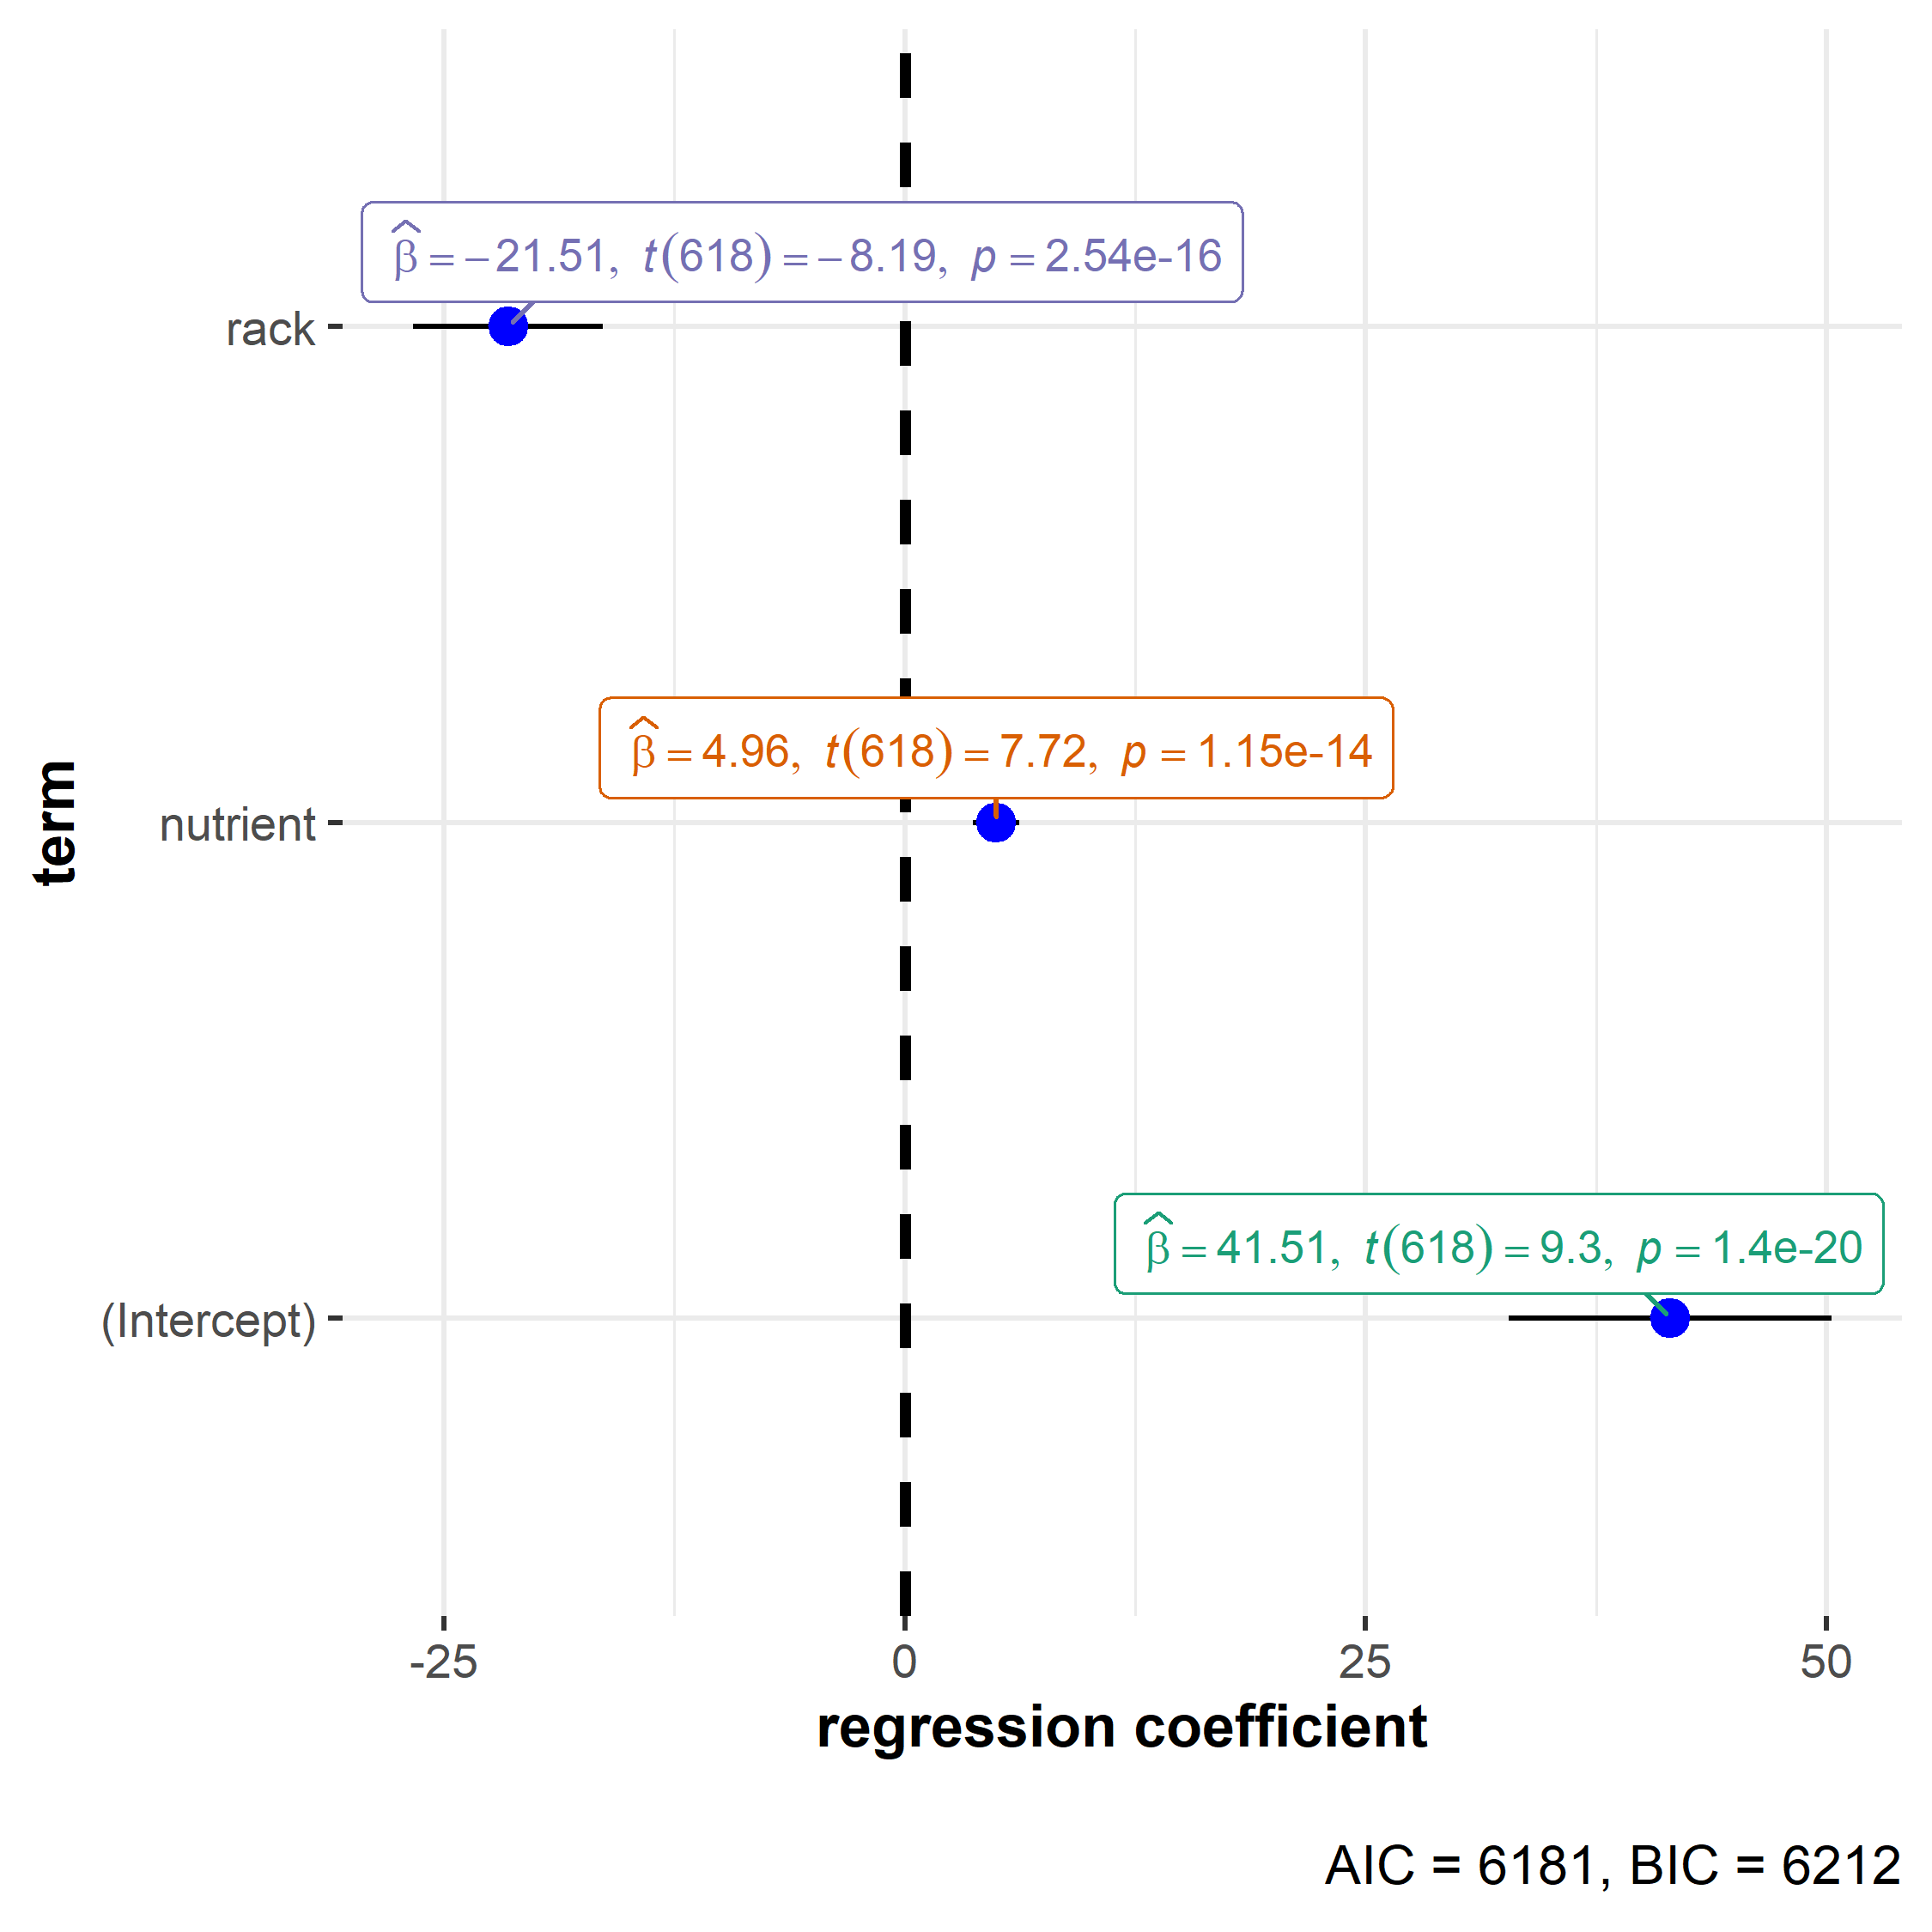
\includegraphics[width=1\linewidth]{./figures/paper-fig6-1} \caption{Sample-to-sample variation in regression estimates is displayed using confidence intervals in `ggcoefstats`.}\label{fig:fig6}
\end{figure}

\hypertarget{statistical-analysis}{%
\section{Statistical analysis}\label{statistical-analysis}}

\hypertarget{data-requirements}{%
\subsection{Data requirements}\label{data-requirements}}

As an extension of \texttt{ggplot2}, \texttt{ggstatsplot} has the same expectations about the
structure of the data. More specifically,

\begin{itemize}
\item
  The data should be organized following the principles of \emph{tidy data}, which
  specify how statistical structure of a data frame (variables and
  observations) should be mapped to physical structure (columns and rows).
  More specifically, tidy data means all variables have their own columns and
  each row corresponds to a unique observation ((\protect\hyperlink{ref-wickhamTidyData2014}{Wickham, 2014})).
\item
  All \texttt{ggstatsplot} functions remove \texttt{NA}s from variables of interest (similar
  to \texttt{ggplot2}; (\protect\hyperlink{ref-wickhamGgplot2ElegantGraphics2016}{Wickham, 2016}), p.207) in the data and
  display total sample size (\emph{n}, either observations for between-subjects or
  pairs for within-subjects designs) in the subtitle to inform the user/reader
  about the number of observations included for both the statistical analysis
  and the visualization. But, when sample sizes differ \emph{across} tests in the
  same function, \texttt{ggstatsplot} makes an effort to inform the user of this
  aspect. For example, \texttt{ggcorrmat} features several correlation test pairs
  and, depending on variables in a given pair, the sample sizes may vary
  (Figure \ref{fig:fig4}).
\end{itemize}

\begin{Shaded}
\begin{Highlighting}[]
\CommentTok{\# for reproducibility}
\FunctionTok{set.seed}\NormalTok{(}\DecValTok{123}\NormalTok{)}

\CommentTok{\# creating a new dataset without any NAs in variables of interest}
\NormalTok{msleep\_no\_na }\OtherTok{\textless{}{-}}
\NormalTok{  dplyr}\SpecialCharTok{::}\FunctionTok{filter}\NormalTok{(}
    \AttributeTok{.data =}\NormalTok{ ggplot2}\SpecialCharTok{::}\NormalTok{msleep,}
    \SpecialCharTok{!}\FunctionTok{is.na}\NormalTok{(sleep\_rem), }\SpecialCharTok{!}\FunctionTok{is.na}\NormalTok{(awake), }\SpecialCharTok{!}\FunctionTok{is.na}\NormalTok{(brainwt), }\SpecialCharTok{!}\FunctionTok{is.na}\NormalTok{(bodywt)}
\NormalTok{  )}

\CommentTok{\# variable names vector}
\NormalTok{var\_names }\OtherTok{\textless{}{-}} \FunctionTok{c}\NormalTok{(}\StringTok{"REM sleep"}\NormalTok{, }\StringTok{"time awake"}\NormalTok{, }\StringTok{"brain weight"}\NormalTok{, }\StringTok{"body weight"}\NormalTok{)}

\CommentTok{\# combining two plots using helper function in \textasciigrave{}ggstatsplot\textasciigrave{}}
\NormalTok{ggstatsplot}\SpecialCharTok{::}\FunctionTok{combine\_plots}\NormalTok{(}
  \AttributeTok{plotlist =}\NormalTok{ purrr}\SpecialCharTok{::}\FunctionTok{pmap}\NormalTok{(}
    \AttributeTok{.l =} \FunctionTok{list}\NormalTok{(}\AttributeTok{data =} \FunctionTok{list}\NormalTok{(msleep\_no\_na, ggplot2}\SpecialCharTok{::}\NormalTok{msleep)),}
    \AttributeTok{.f =}\NormalTok{ ggstatsplot}\SpecialCharTok{::}\NormalTok{ggcorrmat,}
    \AttributeTok{cor.vars =} \FunctionTok{c}\NormalTok{(sleep\_rem, awake}\SpecialCharTok{:}\NormalTok{bodywt),}
    \AttributeTok{cor.vars.names =}\NormalTok{ var\_names,}
    \AttributeTok{colors =} \FunctionTok{c}\NormalTok{(}\StringTok{"\#B2182B"}\NormalTok{, }\StringTok{"white"}\NormalTok{, }\StringTok{"\#4D4D4D"}\NormalTok{),}
    \AttributeTok{title =} \StringTok{"Correlalogram for mammals sleep dataset"}\NormalTok{,}
    \AttributeTok{subtitle =} \StringTok{"sleep units: hours; weight units: kilograms"}
\NormalTok{  ),}
  \AttributeTok{labels =} \FunctionTok{c}\NormalTok{(}\StringTok{"(a)"}\NormalTok{, }\StringTok{"(b)"}\NormalTok{),}
  \AttributeTok{nrow =} \DecValTok{1}
\NormalTok{)}
\end{Highlighting}
\end{Shaded}

\begin{figure}[H]
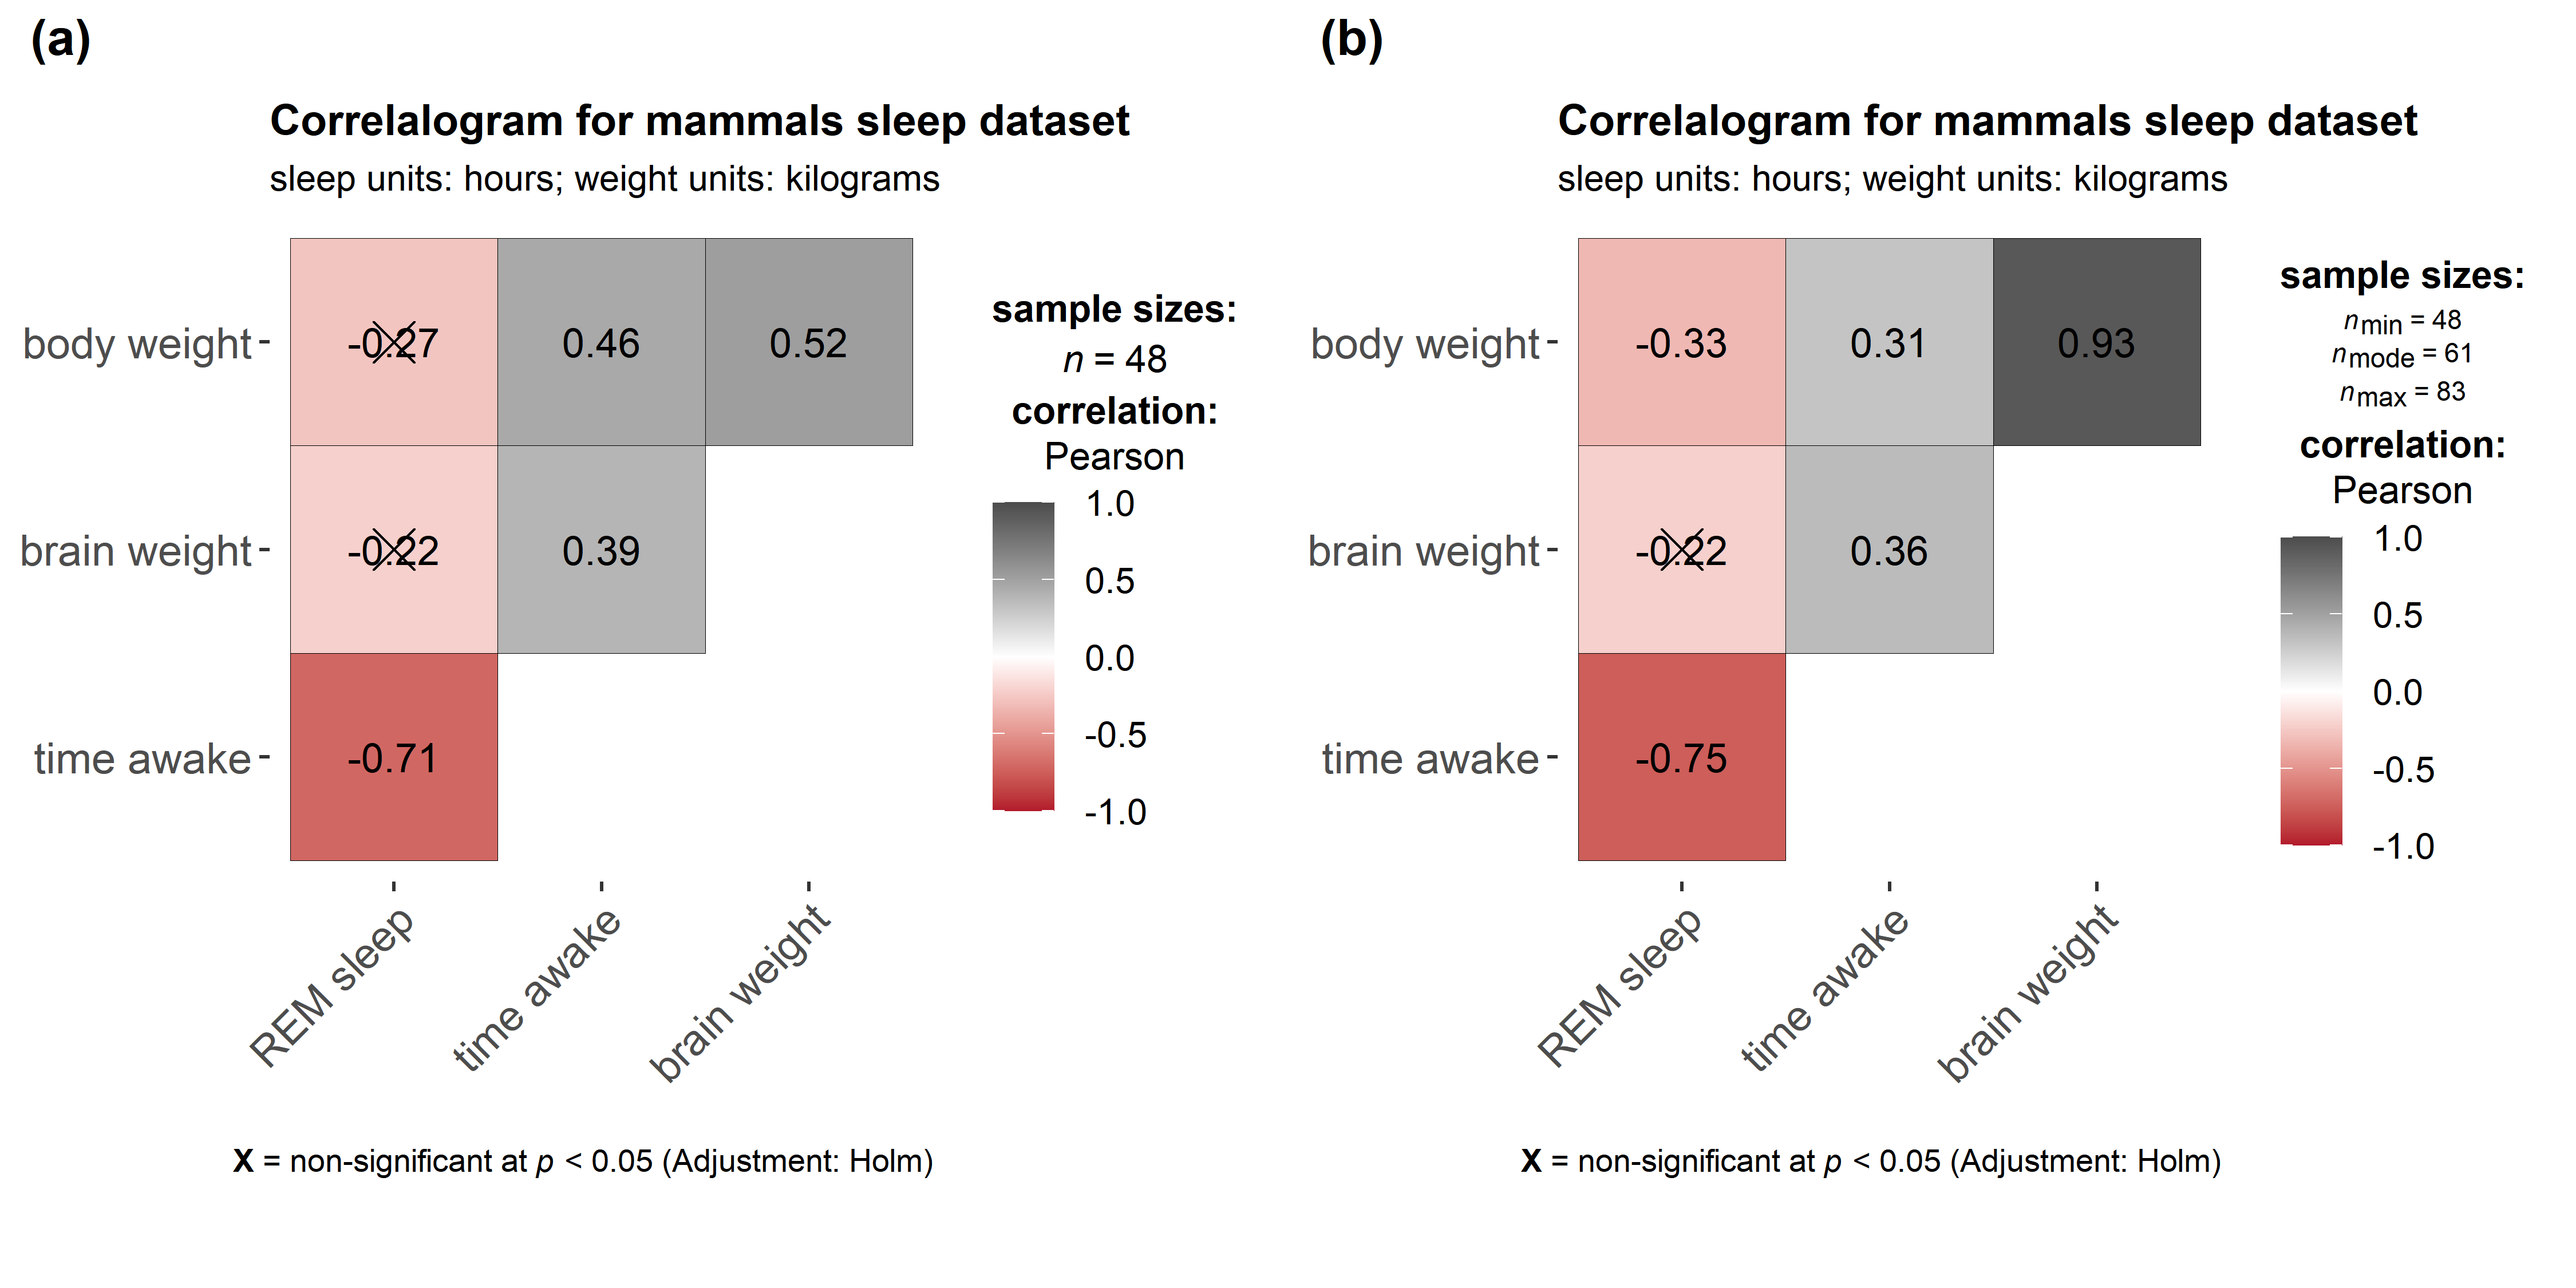
\includegraphics[width=1\linewidth]{./figures/paper-fig4-1} \caption{`ggstatsplot` functions remove `NA`s from variables of interest and display total sample size \textit{n}, but they can give more nuanced information about sample sizes when \textit{n} differs across tests. For example, `ggcorrmat` will display (\textit{a}) only one total sample size once when no `NA`s present, but (\textit{b}) will instead show minimum, median, and maximum sample sizes across all correlation tests when `NA`s are present across correlation variables.}\label{fig:fig4}
\end{figure}

\hypertarget{statistical-reporting}{%
\subsection{Statistical reporting}\label{statistical-reporting}}

The default setting in \texttt{ggstatsplot} is to produce plots with statistical
details included. Most often than not, these results are displayed as a \texttt{subtitle}
in the plot. Great care has been taken into which details are included in
statistical reporting and why. For example, the template below is used to show
results from Yuen's test for trimmed means (robust \emph{t}-test):

\begin{figure}
\centering
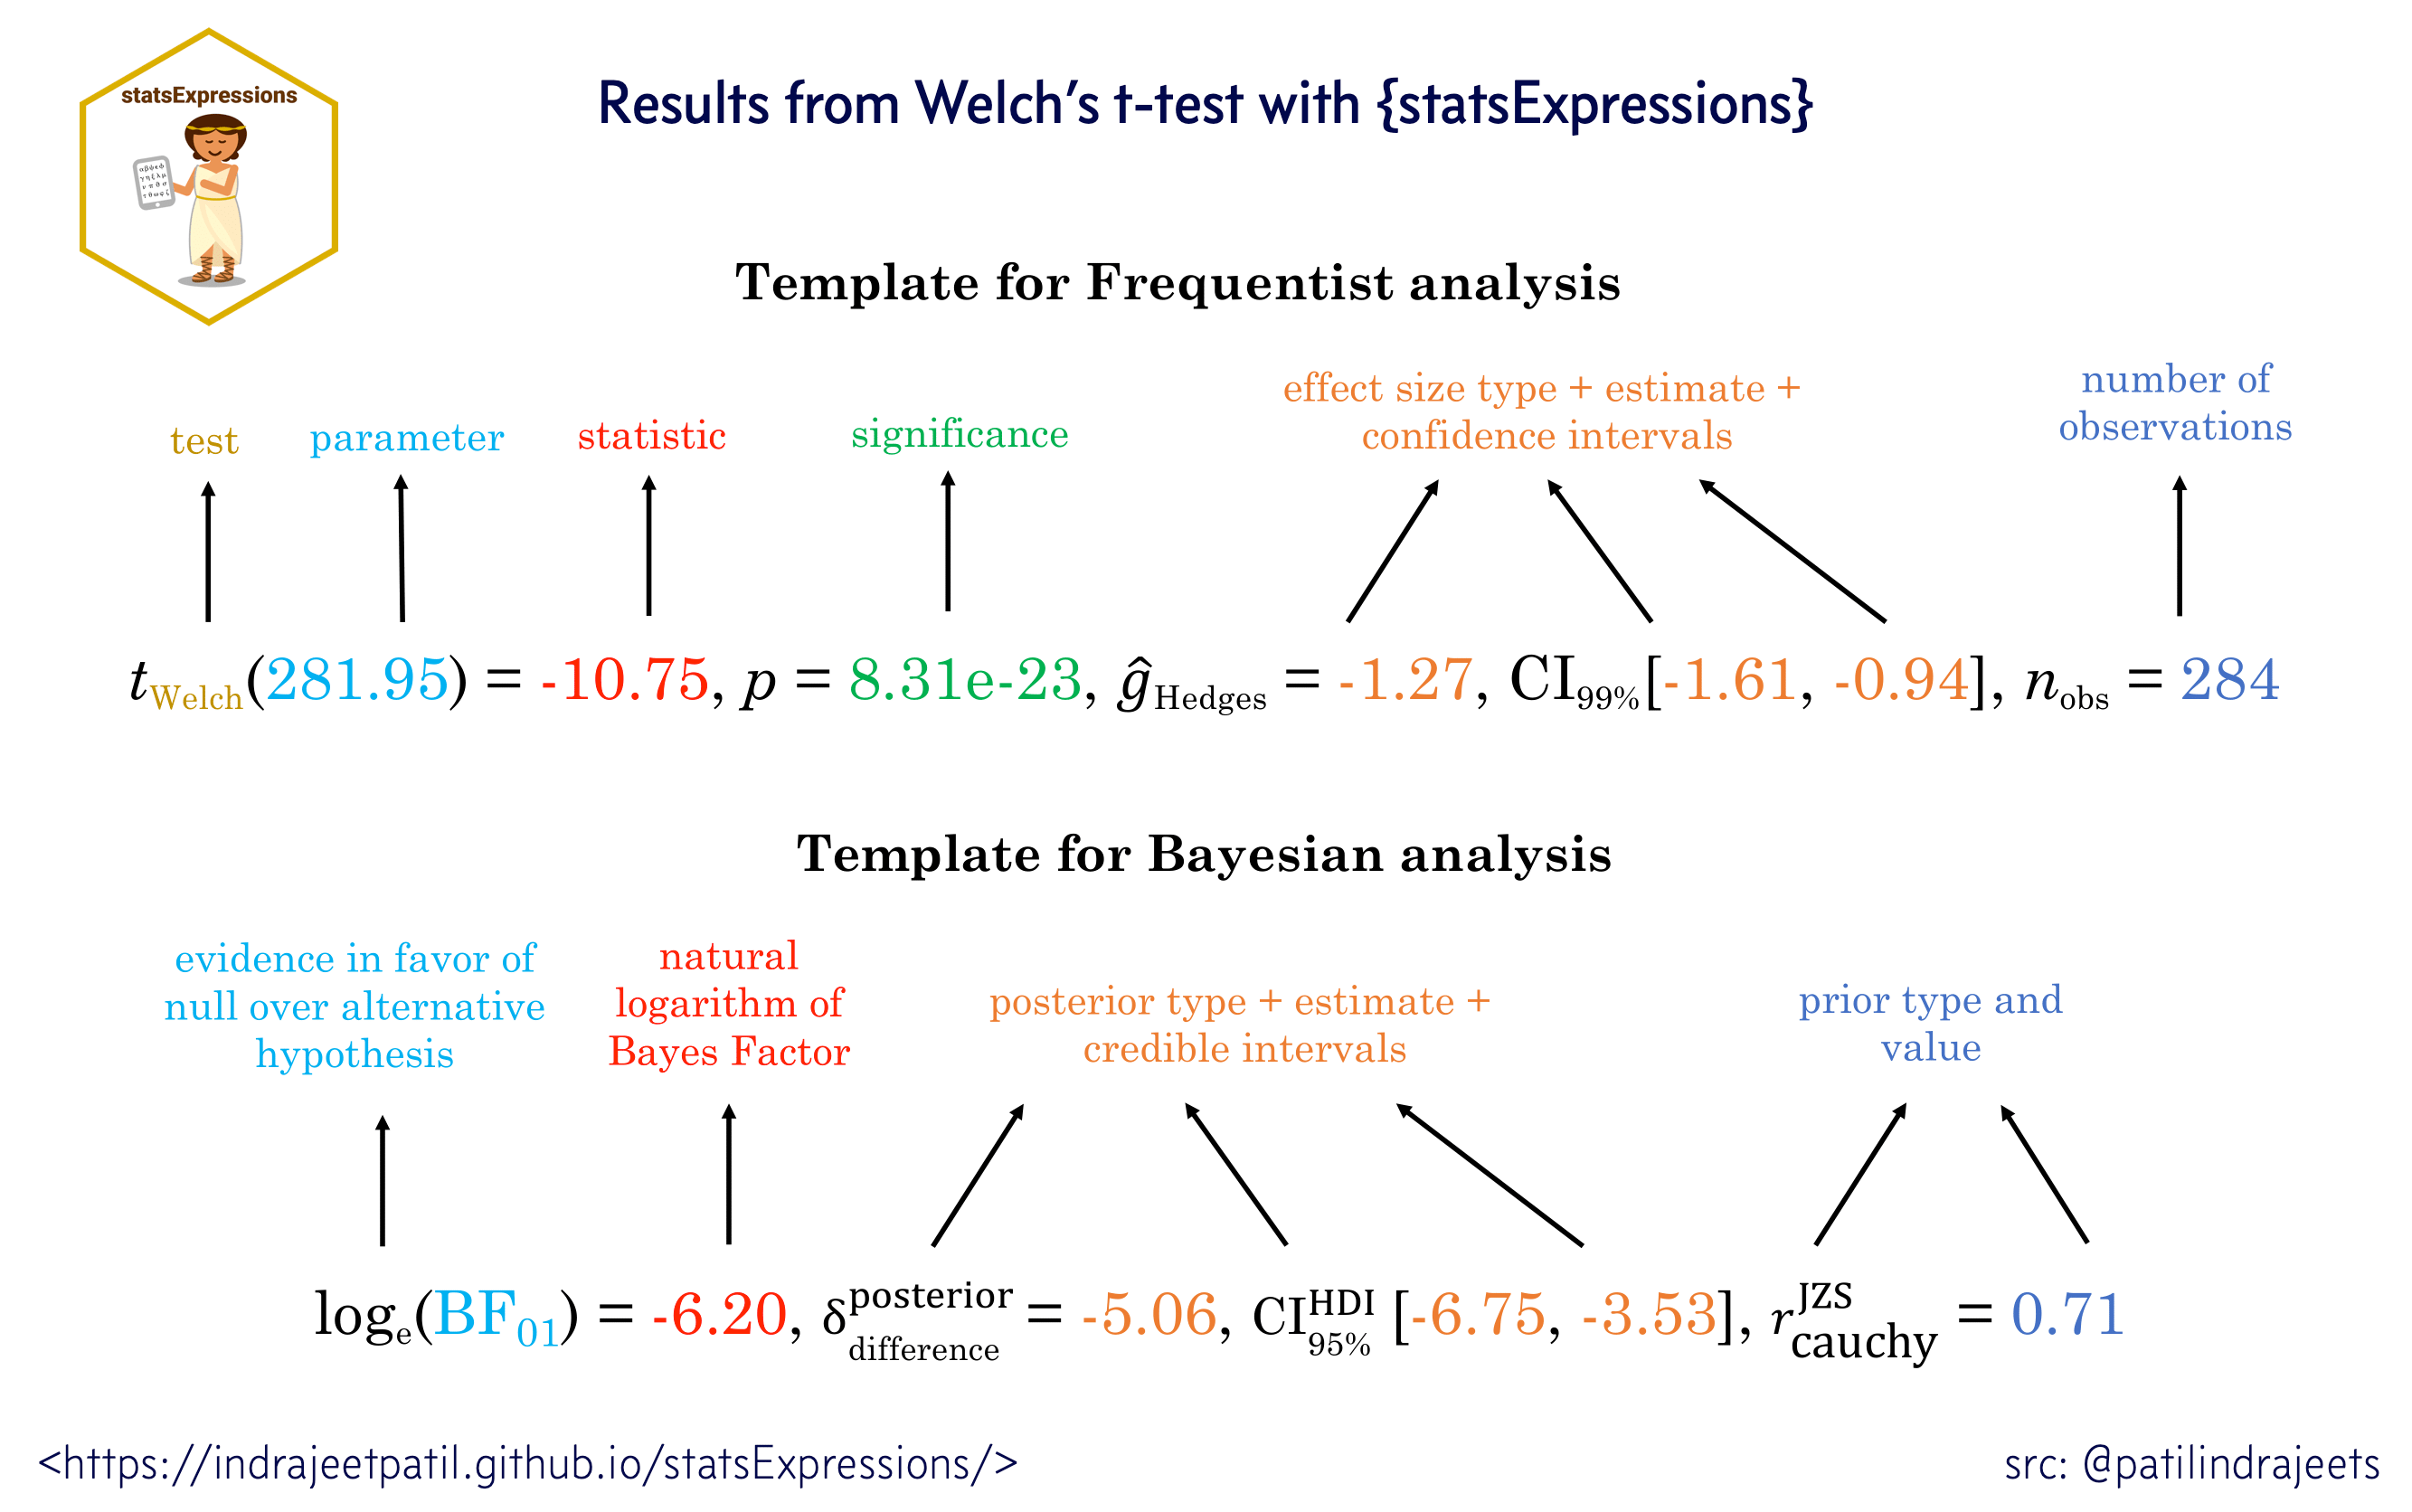
\includegraphics{figures/stats_reporting_format.png}
\caption{Template for reporting statistical details}
\end{figure}

APA guidelines (\protect\hyperlink{ref-associationPublicationManualAmerican2009}{Association, 2009}) are followed by
default while reporting statistical details:

\begin{itemize}
\item
  Percentages are displayed with no decimal places (Figure \ref{fig:fig2}).
\item
  Correlations, \emph{t}-tests, and \(\chi^2\)-tests are reported with the degrees
  of freedom in parentheses and the significance level (Figure \ref{fig:fig4},
  Figure \ref{fig:fig3}, Figure \ref{fig:fig5}).
\item
  ANOVAs are reported with two degrees of freedom and the significance level
  (Figure \ref{fig:fig1}).
\item
  Regression results are presented with the unstandardized or standardized
  estimate (beta), whichever was specified by the user, along with the
  statistic (depending on the model, this can be a \emph{t}, \emph{F}, or \emph{z} statistic)
  and the corresponding significance level (Figure \ref{fig:fig6}).
\item
  With the exception of \emph{p}-values, most statistics are rounded to two decimal
  places by default.
\end{itemize}

\hypertarget{dealing-with-null-results}{%
\subsection{\texorpdfstring{Dealing with \textbf{null results}:}{Dealing with null results:}}\label{dealing-with-null-results}}

All functions therefore by default return Bayes Factor
in favor of the null hypothesis by default. If the null hypothesis can't be
rejected with the null hypothesis significance testing (NHST) approach, the
Bayesian approach can help index evidence in favor of the null hypothesis (i.e.,
\(BF\_{01}\)). By default, natural logarithms are shown because Bayes Factor
values can sometimes be pretty large. Having values on logarithmic scale also
makes it easy to compare evidence in favor alternative (\(BF\_{10}\)) versus null
(\(BF\_{01}\)) hypotheses (since \(log\_{e}(BF\_{01}) = - log\_{e}(BF\_{01})\)).

\hypertarget{avoiding-the-p-value-error}{%
\subsection{\texorpdfstring{Avoiding the \textbf{``p-value error''}:}{Avoiding the ``p-value error'':}}\label{avoiding-the-p-value-error}}

The \emph{p}-value indexes the probability that the researchers have falsely rejected
a true null hypothesis (Type I error, i.e.) and can rarely be \emph{exactly} 0. And
yet over 97,000 manuscripts on Google Scholar report the \emph{p}-value to be \texttt{p\ =0.000},
putatively due to relying on default computer software outputs
(\protect\hyperlink{ref-lilienfeldFiftyPsychologicalPsychiatric2015}{Lilienfeld et al., 2015}). All \emph{p}-values displayed in
\texttt{ggstatsplot} plots avoid this mistake. Anything less than \texttt{p\ \textless{}\ 0.001} is
displayed as such (e.g, Figure \ref{fig:fig1}). The package deems it unimportant how
infinitesimally small the \emph{p}-values are and, instead, puts emphasis on the
effect size magnitudes and their 95\% CIs.

\newpage

\hypertarget{acknowledgments}{%
\section{Acknowledgments}\label{acknowledgments}}

The authors would like to thank all people who have contributed in some way to
the formation of this package. The authors would also like to acknowledge the
help and support provided by the larger \texttt{\#rstats} community on Twitter and
StackOverflow for the development of this package. We also appreciate helpful
discussions with Fiery Cushman.

\newpage

\hypertarget{appendix}{%
\section{Appendix}\label{appendix}}

\hypertarget{appendix-a-documentation}{%
\subsection{Appendix A: Documentation}\label{appendix-a-documentation}}

There are three main documents one can rely on to learn how to use
\texttt{ggstatsplot}:

\begin{itemize}
\item
  \textbf{Presentation}:
  The quickest (and the most fun) way to get an overview of
  the philosophy behind this package and the offered functionality is to go
  through the following slides:
  \url{https://indrajeetpatil.github.io/ggstatsplot_slides/slides/ggstatsplot_presentation.html\#1}
\item
  \textbf{Manual}:\\
  The \texttt{CRAN} reference manual provides detailed documentation about arguments
  for each function and examples:
  \url{https://cran.r-project.org/web/packages/ggstatsplot/ggstatsplot.pdf}
\item
  \textbf{Vignettes}:\\
  Vignettes contain probably the most detailed exposition. Every single
  function in \texttt{ggstatsplot} has an associated vignette which describes in
  depth how to use the function and modify the defaults to customize the plot
  to your liking. All these vignettes can be accessed from the package
  website: \url{https://indrajeetpatil.github.io/ggstatsplot/articles/}
\end{itemize}

\hypertarget{appendix-b-suggestions}{%
\subsection{Appendix B: Suggestions}\label{appendix-b-suggestions}}

If you find any bugs or have any suggestions/remarks, please file an issue on
\texttt{GitHub} repository for this package:
\url{https://github.com/IndrajeetPatil/ggstatsplot/issues}

\hypertarget{appendix-c-session-information}{%
\subsection{Appendix C: Session information}\label{appendix-c-session-information}}

For reproducibility purposes, the details about the session information in which
this document was rendered, see-
\url{https://indrajeetpatil.github.io/ggstatsplot/articles/web_only/session_info.html}

\newpage

\hypertarget{references}{%
\section*{References}\label{references}}
\addcontentsline{toc}{section}{References}

\hypertarget{refs}{}
\begin{CSLReferences}{1}{0}
\leavevmode\hypertarget{ref-associationPublicationManualAmerican2009}{}%
Association, A. P. (2009). \emph{Publication {Manual} of the {American Psychological Association}, 6th {Edition}}. {Washington, DC}: {American Psychological Association}.

\leavevmode\hypertarget{ref-clevelandElementsGraphingData1985}{}%
Cleveland, W. S. (1985). \emph{The {Elements} of {Graphing Data}} (1st edition). {Monterey, Cal}: {Wadsworth, Inc.}

\leavevmode\hypertarget{ref-lilienfeldFiftyPsychologicalPsychiatric2015}{}%
Lilienfeld, S. O., Sauvign'e, K. C., Lynn, S. J., Cautin, R. L., Latzman, R. D., \& Waldman, I. D. (2015). Fifty psychological and psychiatric terms to avoid: A list of inaccurate, misleading, misused, ambiguous, and logically confused words and phrases. \emph{Frontiers in Psychology}, \emph{6}. \url{https://doi.org/10.3389/fpsyg.2015.01100}

\leavevmode\hypertarget{ref-nuijtenPrevalenceStatisticalReporting2016}{}%
Nuijten, M. B., Hartgerink, C. H. J., van Assen, M. A. L. M., Epskamp, S., \& Wicherts, J. M. (2016). The prevalence of statistical reporting errors in psychology (1985{}2013). \emph{Behavior Research Methods}, \emph{48}(4), 1205--1226. \url{https://doi.org/10.3758/s13428-015-0664-2}

\leavevmode\hypertarget{ref-tufteVisualDisplayQuantitative2001}{}%
Tufte, E. R. (2001). \emph{The {Visual Display} of {Quantitative Information}} (2nd edition edition). {Cheshire, Conn}: {Graphics Press}.

\leavevmode\hypertarget{ref-wickhamTidyData2014}{}%
Wickham, H. (2014). Tidy {Data}. \emph{Journal of Statistical Software}, \emph{59}(1), 1--23. \url{https://doi.org/10.18637/jss.v059.i10}

\leavevmode\hypertarget{ref-wickhamGgplot2ElegantGraphics2016}{}%
Wickham, H. (2016). \emph{Ggplot2: {Elegant Graphics} for {Data Analysis}} (2nd ed. 2016 edition). {New York, NY}: {Springer}.

\end{CSLReferences}

\end{document}
